%
%
% you should only have one "documentclass" line.  the following lines
% are samples that give various options.  the nofrontmatter option is
% nice because it suppresses the title and signature pages when you want
% to focus only on the main body of the thesis
%
% Friday April 10 2010 Ray Hylock <ray-hylock@uiowa.edu>
% documentclass options:
%   docabstract				if you want to add a separate doctoral abstract with separate signature page
%   abstractpage            if you want to add an internal abstract (optional)
%	publicabstractpage		if you want to add a public abstract page 
%   ackpage                 if you would like to add an acknowledgements page (optional)
%   algorithms              if you want a list of algorithms (optional)
%   appendix                if you have an appendix (optional)
%   copyrightpage           if you wish to copyright your thesis (optional)
%   dedicationpage          if you wish to make a dedication (optional)
%   epigraphpage            if you would like to add an epigraph to the beginning of your thesis (optional)
%   examples                if you want a list of examples (this uses the ntheorem package)
%   exampleslemmas          if you want a combined list of examples and lemmas (this uses the ntheorem package) (optional)
%   examplestheorems        if you want a combined list of examples and theorems (this uses the ntheorem package) (optional)
%   exampleslemmastheorems  if you want a combined list of examples, lemmas, and theorems (this uses the ntheorem package) (optional)
%   figures                 if you have any figures (this is required if you have even one figure)
%   lemmas                  if you want a list of lemmas (this uses the ntheorem package) (optional)
%   lemmastheorems          ifs you want a combined list of lemmas and theorems (this uses the ntheorem package) (optional)
%   nofrontmatter           suppresses the title and signiture pages for working on the body
%   tables                  if you have any tables (this is required if you have even one table)
%   theorems                if you want a list of theorems (this uses the ntheorem package) (optional)
%   phd                     if phd student; this will add the doctoral abstract (mandatory for PhD and DMA thesis candidates only)
%
\documentclass[abstractpage,publicabstractpage,ackpage,copyrightpage,phd,figures,tables]{uithesis}
\usepackage{amsfonts}
\usepackage{amsmath}
\usepackage{amssymb}
\usepackage{amsthm} % included in ntheorem with amsthm option
%\usepackage[amsthm]{ntheorem} % use if going to make theorem lists
\usepackage{array}
\usepackage{float}
\usepackage[toc,page,titletoc]{appendix}
\usepackage{longtable}
\usepackage{graphicx}
\usepackage[font=singlespacing]{caption}
\usepackage[normalem]{ulem}
\usepackage{nicefrac}
\usepackage{units}
\usepackage{rotating}
\usepackage{afterpage}
\usepackage{tikz}
\usetikzlibrary{arrows,positioning}
\usepackage{tikz-cd}
\usepackage{subcaption}
\usepackage[hidelinks]{hyperref}
\usepackage{cleveref}
\usepackage{multirow}
\usepackage{rotating}
\usepackage{makecell}
%\usepackage[nottoc,notlot,notlof]{tocbibind}

% compress and sort citations as numbers
% alter uithesis.cls line 355 from plain2 to unsrt to use this
%\usepackage[numbers,sort&compress]{natbib}

% does not allow citations to be split between pages; requirement
\usepackage{etoolbox}
\apptocmd{\thebibliography}{\interlinepenalty 10000\relax}{}{}

% Vertical spacing (singlespace) in itemset and enumerate
\usepackage{enumitem}
\setlist{noitemsep,topsep=1pt, partopsep=4pt, parsep=2pt}
\setenumerate{noitemsep,topsep=1pt, partopsep=4pt, parsep=2pt}

% single spacing for rows in a table (this does not single space
% within a row; for that, use \\[-5mm]
\renewcommand\arraystretch{0.5} % 1/2 of the default spacing (double)

\allowdisplaybreaks[2]

% Put user defined commands here
% The \sideremark command is very useful for margin comments

\newcommand{\be}{\begin{enumerate}}
\newcommand{\ee}{\end{enumerate}}

\newtheorem{theorem}{Theorem}[chapter]
\newtheorem{lemma}[theorem]{Lemma}
\newtheorem{corollary}[theorem]{Corollary}
\newtheorem{proposition}[theorem]{Proposition}
\newtheorem{example}[theorem]{Example}
%% math commands
\def \R{\ensuremath \mathbb{R}}
\def \e{\ensuremath \varepsilon}
\def \d{\ensuremath \delta}
\def \tr{\ensuremath \text{tr}}

\theoremstyle{definition}
\newtheorem{defn}[theorem]{Definition}
\newtheorem{remarkalgorithm}[theorem]{Algorithm}
\newtheorem{hypothesis}[theorem]{Hypothesis}

\theoremstyle{remark}
\newtheorem{remark}[theorem]{Remark}

\pdfstringdefDisableCommands{\let\uppercase\relax}

% For figures
\newcommand*{\figuretitle}[1]{
  {\centering
  \textbf{#1}
  \par\medskip}
}
\newcommand*{\figuretitlesmall}[1]{
  {\centering \scriptsize{
  \textbf{#1}
  \par\medskip}}
}


%
% the following command can be used to put a remark
% in the margin of the thesis/paper
% to include a remark, use \edz{remark}
% size of the remark font can be changed, not it
% is set to "scriptsize", can also be "tiny" or "small"
% or others
%
\def\sideremark#1
{
\ifvmode\leavevmode\fi\vadjust
  {\vbox to0pt
    {\vss\hbox to0pt
      {\hskip\hsize\hskip1em\vbox
        {\hsize2cm
%          \small
          \scriptsize
          \raggedright\pretolerance10000\noindent#1\hfill
        }
        \hss
      }
      \vbox to8pt{\vfil}\vss
    }
  }
}


% !Tex root = thesis.tex

% This is the prelude to my thesis and contains much of what is needed to
% create my thesis


%% Front Matter %%%%%%%%%%%%%%%%%%%%%%%%%%%%%%%%%%%%%%%%%%%%%%%%%%%%%%%%
%\abtitlepgfalse       % print out the microfiche title page
%\abstractpgfalse      % print out the microfiche abstract
% \abtitlepgtrue       % print out the microfiche title page
% \abstractpgtrue      % print out the microfiche abstract

%\titlepgtrue          % print out the title page
%\copyrightfalse       % claim my true inheritance
%\signaturepagetrue    % page for thesis committee members
%\dedicationtrue       % page for the dedication
%\acktrue              % Print out the acknowledgements
%\abswithesisfalse     % abstract for the thesis
%\tablecontentstrue    % page for table of contents
%\figurespagefalse     % page of figures
%%%%%%%%%%%%%%%%%%%%%%%%%%%%%%%%%%%%%%%%%%%%%%%%%%%%%%%%%%%%%%%%%%%%%%%%%

%%%%% TITLE %%%%%%%%%%%%
%\title{Developing Machine Learning Algorithms for Application in Educational Measurement}
\title{Neural Network Methods for Application in \\ Educational Measurement}

%%%%%%%%% AUTHOR %%%%%%%%%%%%
\author{Geoffrey Converse}
%%%%%%%%% Other Stuff %%%%%%%%%%%%
\dept{Applied Mathematical and Computational Sciences}
% for a single advisor
\setboolean{multipleSupervisors}{false}
\advisor{\\Professor Suely Oliveira} %  \hspace{56mm} Second Advisor Title and Name}
% for multiple advisors; change <value> to line up the names
%\setboolean{multipleSupervisors}{true}
%\advisor{Advisor 1\\\hspace{4mm}Advisor 2...}
%
% edit the names below to have your committee members names appear
% on the signature page.  memberOne should be your advisor.
%
\memberOne{Suely Oliveira}
\memberTwo{Mariana Curi}
\memberThree{David Stewart}
\memberFour{Jonathan Templin}
\memberFive{Colleen Mitchell}
% Comment in if there are six committee members, also need to comment in two commands in thesis.cls, search "six committee members" to find where to comment in commands in thesis.cls
%\memberSix{Member Six}

\submitdate{August 2021}
\copyrightyear{2021}


% Abstracts for the various purposes
%\newcommand{\abstextwithesis}{\myabstract}
%\newcommand{\abstracttext}{\myabstract}

% Dedication for the thesis.
%\epigraph{epigraph}
%\dedication{dedication}

% Acknowledgement file
\ackfile{thesisAck}
% Abstract file - specifies the text for the abstract.  This is used
% in the PhD Abstract, as well as in the abstract bounded with
% the dissertation
\abstractfile{thesisAbstract}
\publicabstractfile{thesisAbstractpublic}


       % Front matter, title page, etc.

\begin{document}

% Puts some of the front matter in

\frontmatter

% Include the chapters and appendix here

% !Tex root = thesis.tex

% Chapter One - Chapter One Title
\chapter{Chapter Title} \label{label}

This is the first chapter of the thesis. Here is how to cite a reference \cite{thissen}. You can use $\backslash$Cref\{label\} \Cref{label} to reference a chapter, section, theorem, etc. Also, $\backslash$sideremark\{text\} \sideremark{Here is a comment in the margin} allows you to make remarks in the margin for editing purposes. 

\section{Background - IRT Parameter Estimation}
In educational measurement, a common goal is to quantify the knowledge of students from the results of some assessment. In a classroom setting, grades are typically assigned based on the percentage of questions answered correctly by a student assignments. The letter grades assigned from these percentages can serve as a naive measure of student knowledge; ``A'' students have completely mastered the material, ``B'' students have a good grasp of material, ``C'' students are fairly average, and ``D'' and ``F'' students have significant gaps in their knowledge.

The practice of evaluating student ability purely from a raw percentage score is known as true score theory \parencite{thissen} \cite{thissen} ~\textcite{thissen}. But there are clear issues with this approach. Not all questions on an exam or homework assignment is created equally: some questions are easier, and some more difficult. Consider a scenario where two students both answer 17 out of 20 questions correctly on a test for a raw score of $85\%$. But if Student A answered questions 1, 8, and 9 wrong while Student B answered 4, 17, and 20 incorrectly, it is not likely that that Student A and Student B possess the same level of knowledge. For example, questions 1, 8, and 9 could be much more difficult than questions 4, 17, and 20. Additionally, the two sets of problems could cover different types of material. True score theory does not account for either of these situations, and naively quantifies the knowledge of Student A and Student B as equal.

More sophisticated methods have been studied which attempt to more accurately quantify student learning. Cognitive Diagnostic Models (CDM) (TODO: citation) aim to classify whether students possess mastery of a given skill or not. This discrete classification can be useful in determining whether or not a student meets a prerequisite, or deciding whether or not they are ready to move on to the next level of coursework. We focus instead on Item Response Theory, where student knowledge is assumed to be continuous.

\subsection{Item Response Theory}
Item Response Theory (IRT) is a field of quantitative psychology which uses statistical models to model student ability. These models often give the probability of a question being answered correctly as a function of the student's ability.

\subsubsection{Rasch Model}

\subsubsection{The method with the integral thing}

\subsubsection{2-Parameter Logistic Model}

\subsection{Parameter Estimation Methods}

\subsection{Artificial Neural Networks}
In recent years, artifical neural networks (ANN) have become an increasingly popular tool for machine learning problems. Though they have been around since the 1960's (TODO: citation), GPU technology has become more accessible and modern computers are more powerful, allowing anyone interested to train a basic neural network on their machine. ANN can be applied to a diverse set of problems, including regression, classification, computer vision, natural language processing, function approximation, data generation, and more (TODO: citations).

One of the biggest critiques of ANN is their black-box nature, meaning that the decision process that a trained model uses is typically not explainable by humans. As opposed to simpler methods such as decision trees or linear regression, neural networks are not interpretable. This makes them less desirable in certain applications where researchers wish to know \textit{why} a model predicts a particular data sample the way that it does. For example, if a financial institution is using data science methods to determine whether or not to approve someone's loan, the institution should be able to explain to the customer why they were denied. Most customers will not be satisfied with ``the computer told us so,'' and there is a possibility that a black-box neural network could learn and use features such as race or gender in its prediction, which is illegal in the United States (TODO: definitely need citation or delete).

\subsubsection{Autoencoders}

\subsubsection{Variational Autoencoders}


\end{center}

\chapter{Estimating IRT Parameters with Variational Autoencoders}
The primary contribution of this thesis is the development of a method for IRT parameter estimation which uses a modified VAE. The method, titled ``ML2P-VAE'', is interesting from multiple perspectives. In the application area, it is an unconventional approach can produce estimates as accurate as those of traditional parameter estimation techniques. Further, ML2P-VAE scales much better than traditional methods as the number of latent abilities becomes large. In the field of machine learning, ML2P-VAE is an unsupervised learning technique which yields explainable results. A variational autoencoder is used in an unorthodox way, and the trainable parameters and a hidden neural layer are able to be understood in a real-world context.

\section{ML2P-VAE Method Description}\label{sec:ml2p_vae}
Assume we are given an assessment with $n$ items which tests $K$ latent skills, and that $N$ students take this exam. Data is given as an $N \times n$ binary matrix, as in Equation \ref{eq:responses}. No information about student latent ability parameters $\Theta \in \R^K$ or item parameters $a_{ik}$ and $b_i$ is provided. However, there is access to an expert-annotated binary $Q$-matrix detailing the item-skill associations, as in Equation \ref{eq:q_matrix}.

\sideremark{TODO: relate to IRT background section and VAE derivation}

A number of specifications are required in order to use a VAE as an IRT parameter estimation method. First, set up the neural network so that the input and output layers each have $n$ nodes, each representing one item. The inputs are be the binary response vectors $\vect u_j$ and the outputs are approximations of the probability of student $j$ answering each item correctly. Next, the dimension of the hidden distribution (the output of the encoder) must be equal to $K$, the number of latent skills. The usual VAE loss function described in Equation \ref{eq:vae_loss} is still used to optimize ML2P-VAE.
The modifications to a typical VAE architecture are focused on the decoder. No hidden layers are used in the decoder. Instead, a non-dense set of weights connects the decoder input to the decoder output. The non-zero weights here are determined by the $Q$-matrix; recall that the input to the decoder has $K$ nodes, the decoder output has $n$ nodes, and $Q \in \{0,1\}^{n \times K}$. So for a trainable weight $w_{ik}$ in the VAE decoder, if $q_{ik}=0$, then fix $w_{ik}=0$ as well, and it will never be updated during the training process. This modification is key to allowing interpretation of the hidden latent distribution of a VAE.

The ML2P-VAE method requires the use of the sigmoid activation function
\begin{equation}
  \sigma(z_i) = \frac{1}{1 + e^{z_i}}
  \label{eq:sigmoid}
\end{equation}
in the output layer. Here, $z_i = \sum_{k=1^K} w_{ik}\alpha_{k} + \beta_i$, where $w_{ik}$ is the weight between the $k$-th and $i$-th nodes in the decoder input and decoder output layer, $\alpha_k$ is the activation of the $k$-th node in the decoder input layer, and $\beta_i$ is the additive bias in the output layer. Note the similarity between Equation \ref{eq:sigmoid} and Equation \ref{eq:ml2p}. The constraint on the weights along with the sigmoid activation function allows for interpretation of the decoder as an ML2P model.

Specifically, the decoder weights $w_{ik}$ can be interpreted as estimates to the discrimination parameters $a_{ik}$, the output bias $\beta_i$ can be interpreted as estimates to the difficulty parameters $b_i$, and the activations $\alpha_k$ produced by the encoder (given response input $\vect u_j$) can be interpreted as estimates to the student ability parameter $\theta_{kj}$. \sideremark{may want to mention that the value outputted by encoder is then sampled from for decoder input}

Further modifications can improve the performance of ML2P-VAE. In IRT, discrimination parameters are assumed to be non-negative, because an increase in a skill should never decrease the probability of answering an item correctly. With this assumption in mind, requiring all decoder weights $w_{ik} \geq 0$ avoids a potential identification problem. \sideremark{explain what this means $-\theta a_{ik} = \theta (-a_{ik})$}

Relating the ML2P-VAE model back to the derivation of a variational autoencoder in Section \ref{sec:vae_derive}, the notations used are related as follows. The response vectors $\vect u_j$ serve as the observed data $\vect x$, and the latent ability of students $\vect \Theta_j$ serve as the latent code $\vect z$. The modified decoder, which produced outputs the probabilities of student $j$ answering item $i$ correctly $\hat P_{ij} = \sigma(\theta_{ij})$, as described in Equation \ref{eq:sigmoid}, serves as the observed input reconstruction $\hat x_i$ in Equation \ref{eq:bernoulli}.

\subsection{Full Covariance Matrix Implementation}\label{sec:cov}
There are many publicly available code examples of VAE implementations which assume the latent space follows a standard normal distribution $\mathcal{N}(0,I)$. But it is not so common to train a VAE which assumes the latent prior $p(\Theta)$ has correlated dimensions. Since most applications do not attempt to interpret hidden layers of a VAE, there is no available information on the correlations of abstract, unobservable features. Additionally, it is often beneficial to force the latent dimensions to be independent of one another.

In IRT, we may be able to quantify the correlation between latent abilities, presenting need for the ML2P-VAE model to take advantage of this information. This task is nontrivial due to two mechanisms of the VAE:
\begin{itemize}
  \item[(1)] sampling from the learned distribution, and
  \item[(2)] calculating Kullback-Leibler Divergence
\end{itemize}
These two characteristics must be addressed when constructing the neural architecture.

After training a VAE, sending a data point $u_0$ through the encoder needs to give a set of values that correspond to a probability distribution. For a $K$-dimensional multivariate Gaussian distribution, these values are a vector $\mu_0 \in \R^K$ and a symmetric, positive-definite matrix $\Sigma_0 \in \R^{K\times K}$. Sampling from $\mathcal{N}(\mu_0, \Sigma_0)$ requires a matrix $G_0$ such that $G_0 G_0^\top = \Sigma_0$. This matrix factorization $G_0$ is not unique, but it can be convenient to use the Cholesky decomposition of $\Sigma_0$ \cite{atkinson}. The sample of the multivariate Gaussian is calculated as $z_0 = \mu_0 + G_0 \vect{\e_0}$, where $\vect{\e_0} = (\e_1, \ldots, \e_K)^\top$ and $\e_i \sim \mathcal{N}(0,1)$. 

The KL-Divergence between two $K$-variate Gaussian distributions is given as
\begin{equation}
\begin{split}
  &\mathcal{D}_{KL}\left[\mathcal{N}(\mu_0, \Sigma_0) || \mathcal{N}(\mu_1, \Sigma_1) \right] = \\
&\frac{1}{2} \left( \tr(\Sigma_1^{-1}) \Sigma_0) + (\mu_1 - \mu_0) \Sigma_1^{-1} (\mu_1 - \mu_0) - K + \ln\left( \frac{\det \Sigma_1}\det \Sigma_0 \right) \right)
  \label{eq:kl_multivariate}
\end{split}
\end{equation}
When using this in a VAE, $\mathcal{N}(\mu_1, \Sigma_1)$ corresponds to the prior $p(\Theta)$, and so $\mu_1$ and $\Sigma_1$ are constant. Then $\Sigma_1^{-1}$ only needs to be computed once, and this matrix inversion won't cause computation time problems at any point. Note that Equation \ref{eq:kl_multivariate} computes $\ln \det \Sigma_0$, so we must have $\det \Sigma_0 > 0$ at any point during training. Recall that $\mu_0$ and $\Sigma_0$ correspond to the input $u_0$, and also depend on all the trainable weights and biases in the VAE encoder. These parameters are usually initialized randomly, and the user has little control over their values during training. If $\det \Sigma_0 \leq 0$ for any input $u_0$ at any point during training, then it is not possible to compute the loss and gradient. Thus, a specific architecture which guarantees that $\det \Sigma_0 > 0$, regardless of the input $u_0$ or encoder parameters, is required.

This architecture is described as follows. The input and output to the neural network consists of $n$ nodes, each representing an item on an assessment. After a sufficient number of hidden layers of sufficient size, the encoder outputs $K + \frac{K(K+1)}{2}$ nodes. The first $K$ nodes represent the mean vector $\mu_0$, and the remaining $\frac{K(K+1)}{2}$ nodes are arranged into a lower triangular matrix $L_0 \in \R^{K\times K}$. The covariance matrix is obtained by using the matrix exponential $\Sigma_0 = e^{L_0} \cdot \left( e^{L_0} \right)^\top$.

\begin{theorem}
  $\Sigma_0$ constructed as described previously is symmetric, positive-definite, and has positive determinant.
  \label{thm:cov_vae}
\end{theorem}
\begin{proof}
  Consider any lower triangular $L_0 \in \R^{K\times K}$. Define 
  \[G_0 = e^{L_0} = \sum_{n=1}^\infty \frac{L_0^n}{n!} = I + L_0 + \frac{1}{2} L_0 \cdot L_0 + \cdots\]
  $G_0$ is lower triangular, since addition and multiplication of matrices preserve this property. Further, $G_0$ is nonsingular, because $\det G_0 = \det(e^{L_0}) = e^{\tr L_0} > 0$.

  Set $\Sigma_0 = G_0 G_0^\top$. Clearly, $\Sigma_0$ is symmetric as $\Sigma_0^\top = (G_0 G_0^\top)^\top = G_0 G_0^\top = \Sigma_0$. Further, $\det \Sigma_0 = \det G_0 \cdot \det G_0^\top > 0$. So now for any nonzero $x \in \R^K$,
  \[\langle \Sigma_0 x, x \rangle = x^\top \Sigma_0 x = x^\top G_0 G_0^\top x = \langle G_0^\top x, G_0^\top x \rangle = ||G_0 x||_2^2 > 0\]
  Therefore, $\Sigma_0$ is positive-definite.
\end{proof}

Theorem \ref{thm:cov_vae} shows that in this specific neural network architecture, $\Sigma_0$ can be interpreted as a covariance matrix. Thus, the VAE encoder maps a data point $u_0$ to a multivariate Gaussian distribution $\mathcal{N}(\mu_0, \Sigma_0)$. Additionally, the sampling operation and KL-Divergence calculation can always be carried out without issue. A visualization of the ML2P-VAE architecture for correlated latent traits is shown in Figure \ref{fig:ml2pvae_visual}.

\begin{figure}[h]
  \centering
  \includegraphics[width=.85\textwidth]{img/ml2pvae_visual.png}
  \caption{Visualization of the ML2P-VAE architecture for two correlated latent traits and six input items. Note that the trainable weights matrix in the decoder is not dense, but is determined by the given $Q$-matrix.}
  \label{fig:ml2pvae_visual}
\end{figure}


\subsection{Variants of ML2P-VAE}\label{sec:variants}

We consider three scenarios for using ML2P-VAE in practice: (a) the best case scenario where we assume that the covariance matrix between all latent traits is known, (b) we don't know the exact covariance matrix, so it is estimated using other methods, and (c) we simply assume that all traits are independent. These three situations result in three variations of the ML2P-VAE method: ML2P-VAE$_{full}$, ML2P-VAE$_{est}$, and ML2P-VAE$_{ind}$, respectively. 

In scenario (b), we multiply the response matrix ($N$ students by $n$ items) by the $Q$-matrix ($n$ items by $K$ abilities). We then take the Pearson correlation of the columns of this $N\times K$ matrix to obtain an approximate correlation matrix in $\R^{K\times K}$ between abilities.

In order to estimate the correlations between latent traits for use of ML2P-VAE$_{est}$, the student response matrix $U \in \R^{N\times n}$ is multiplied by the $Q$-matrix $Q \in \R^{n \times K}$. Then the Pearson correlation of the columns of the resulting matrix produce an approximate correlation matrix $\hat \Sigma \in \R^{K \times K}$: 
\[M = U \cdot Q , \quad M \in \R^{N\times K}\]
\begin{equation}
  \hat \Sigma_{kl} = \frac{\sum_{i=1}^N (k_i - \bar k)(l_i - \bar l)}{\sqrt{\sum_{i=1}^N(k_i - \bar k)^2} \sqrt{\sum_{i=1}^N (l_i - \bar l)^2}}
  \label{eq:approx_cor_mat}
\end{equation}
where $\bar k$ and $\bar l$ are the mean values of the $k$-th and $l$-th columns of $M$, respectively.

A final variation of ML2P-VAE comes when the IRT model to be estimated is changed. If assuming that student responses are generated according to the Rasch model as in Equation \ref{eq:rasch}, rather than the ML2P model as in Equation \ref{eq:ml2p}, then another variation of VAE parameter estimation methods can be considered. A more appropriate name for this alternative estimation method is Rasch-VAE.

Since there are no discrimination parameters in the Rasch model, only item difficulties and student abilities need to be estimated. To account for this, the weights in the VAE decoder are restricted to be \textit{equal} to the $Q$-matrix. This still allows for interpretation of the learned distribution of the VAE as estimates to student abilities $\Theta$, while requiring ``discrimination parameters'' to be equal to either one or zero, fitting more closely to Equation \ref{eq:rasch}.

%\subsection{On Convergence}
%
%\subsubsection{Proving local minimum at true solution}
%\sideremark{Can't really guarantee convergence globally with SGD because neural nets are super nonconvex}
%
%In this section, we investigate how the modified ML2P-VAE model fits into the theoretical derivation of a VAE, as described in Section \ref{sec:vae_derive}.
%
%We define the true and predicted probability of student $j$ answering item $i$ correctly with $P_{ij}$ and $\hat P_{ij}$, respectively. The former comes from the ML2P model, and the latter is the output of a neural network as in Equation \ref{eq:sigmoid}. We assume the more simple case, where $\Theta \sim \mathcal{N}(0,I)$, rather than $\mathcal{N}(\mu, \Sigma)$.
%\begin{equation}
%  P_{ij} = \frac{1}{1 + \exp\left(-\sum_{k=1}^K a_{ik}\theta_{jk} + b_i\right)}
%  \label{eq:ml2p_est}
%\end{equation}
%
%\begin{equation}
%  \hat P_{ij} = \frac{1}{1 + \exp\left(-\sum_{k=1}^K \hat a_{ik} (\hat \theta_{jk} + \e_k \hat \sigma_k) + \hat b_i\right)} 
%    \label{eq:vae_out}
%\end{equation}
%
%Note that $P_{ij}$ is unknown, and we instead have a response sequence $\vect u_j = (u_{1j},\ldots, u_{nj})^\top$ with $u_{ij} = \text{Bern}(P_{ij})$. This also means that $\mathbb{E}[u_{ij}] = P_{ij}$. The variables $\hat a_{ik}$, $\hat b_i$, $\hat \theta_{ik}$, and are parameter estimates from the VAE. The first two are parameters in the neural network, and the ability estimates are taken from feeding responses to the encoder, i.e., $\hat \Theta_j = \text{Encoder}(\vect u_j)$. The noise $\e = (\e_k)_{1\leq k \leq K} \sim \mathcal{N}(0,I)$ is introduced by the sampling operation in the VAE.
%
%\sideremark{Instead of VAE loss (which is really ELBO), this should be the marginal prob. of data (see Kingma/Welling)}
%
%The loss function for a VAE is given by 
%\begin{equation}
%  \begin{split}
%  \mathcal{L}(\vect u_j) &= -\sum_{i=1}^n \left[u_{ij} \log(\hat P_{ij}) + (1-u_{ij})\log(1 - \hat P_{ij})\right] + \mathbb{E}_{q_\alpha(\hat \theta | \vect u_j)}\log\left( \frac{q_{\alpha}(\hat \theta |\vect u_j)}{p(\theta)}\right) \\
%    &= \mathcal{L}_{\text{REC}} + \mathcal{L}_{\text{KL}}
%  \end{split}
%  \label{eq:vae_loss}
%\end{equation}
%We break up the VAE loss into two terms, the reconstruction loss $\mathcal{L}_{\text{REC}}$ and the KL-divergence loss $\mathcal{L}_{\text{KL}}$. in the latter, the distribution $q_\alpha(\hat \theta | \vect u_j)$ is the output of the encoder, and $p(\theta)$ is the assumed prior distribution of $\Theta$, which we set to be $\mathcal{N}(0,I)$.
%
%We write $P_{ij} = \mathbb{E}(u_{ij})$, and similarly define a new ``expected'' loss function:
%\begin{equation}
%  \begin{split}
%  \mathcal{L}_\mathbb{E}(P_j) &= \mathbb{E}_{u_j}[\mathcal{L}(u_{:j})] \\
%  &= -\sum_{i=1}^n [P_{ij} \log(\hat P_{ij}) + (1-P_{ij})\log(1 - \hat P_{ij})] + \mathbb{E}_{q_\alpha(\hat \theta | u_j)}\log\left( \frac{q_{\alpha}(\hat \theta |u_j)}{p(\theta)}\right) \\
%    &= \mathcal{L}_{\mathbb{E}[\text{REC}]} + \mathcal{L}_{\mathbb{E}[\text{KL}]}
%  \end{split}
%  \label{eq:expected_loss}
%\end{equation}
%Notice that calculation of this ``expected loss'' requires the unknown $P_{:j}$. But when we have large amounts of data, we can think of $P_{ij}$ as the average value of the response $u_{ij}$, so using this unknown value here is justified.
%
%Define $z_i = a_{i:} \cdot \theta_{j:} - b_i$ and $\hat z_i = \hat a_{i:} \cdot (\hat \theta_{j:} + \e \cdot \hat \sigma) - \hat b_i$. Note that $z_i$ is fixed, dependent on the data, and does not depend on any parameters of the neural network. $\hat z_:$ is the input to the final layer of the decoder, and the VAE output is $\hat P_{ij} = \sigma(\hat z_i)$, where $\sigma(\cdot)$ is the sigmoid activation function. We compute derivatives of the expected loss function, looking individually at the reconstruction and KL terms. 
%
%\begin{equation}
%  \begin{split}
%  \frac{\partial \mathcal{L}_{\mathbb{E}[\text{REC}]}}{\partial \hat z_i} &= \frac{-1}{1 + e^{-z_i}}\cdot \frac{1}{1 + e^{\hat z_i}} - \frac{1}{1 + e^{z_i}}\cdot \frac{-1}{1 + e^{-\hat z_i}} \\
%  &= \frac{-1}{(1 + e^{-z_i})(1 + e^{\hat z_i})} + \frac{1}{(1 + e^{z_i})(1 + e^{-\hat z_i})} \\
%  &= \frac{-1}{(1 + e^{-a_{i:} \cdot \theta_{j:} + b_i})(1 + e^{\hat a_{i:} \cdot (\hat \theta_{j:} + \e_: \hat \sigma_:) - \hat b_i})} \\
%  &\quad + \frac{1}{(1 + e^{a_{i:} \cdot \theta_{j:} - b_i})(1 + e^{-\hat a_{i:} \cdot (\hat \theta_{j:} + \e_: \hat \sigma_:) + \hat b_i})} 
%\end{split}
%  \label{eq:z_deriv}
%\end{equation}
%
%
%\begin{equation}
%  \begin{split}
%  \frac{\partial \mathcal{L}_{\mathbb{E}[\text{REC}]}}{\partial \hat a_{ik}} &= 
%  \frac{\partial \mathcal{L}_{\mathbb{E}[\text{REC}]}}{\partial \hat z_i}\frac{\partial \hat z_i}{\partial \hat a_{ik}} = \frac{\partial \mathcal{L}_{\mathbb{E}[\text{REC}]}}{\partial \hat z_i} (\hat \theta_{jk} + \e_k \hat \sigma_k) \\
%  \frac{\partial \mathcal{L}_{\mathbb{E}[\text{REC}]}}{\partial \hat b_i} &= 
%  \frac{\partial \mathcal{L}_{\mathbb{E}[\text{REC}]}}{\partial \hat z_i}\frac{\partial \hat z_i}{\partial \hat b_i} = \frac{\partial \mathcal{L}_{\mathbb{E}[\text{REC}]}}{\partial \hat z_i} (-1) \\
%  \frac{\partial \mathcal{L}_{\mathbb{E}[\text{REC}]}}{\partial \hat \theta_{ik}} &= 
%  \frac{\partial \mathcal{L}_{\mathbb{E}[\text{REC}]}}{\partial \hat z_i}\frac{\partial \hat z_i}{\partial \hat \theta_{ik}} = \frac{\partial \mathcal{L}_{\mathbb{E}[\text{REC}]}}{\partial \hat z_i} (\hat a_{ik}) 
%\end{split}
% \label{eq:param_deriv}
%\end{equation}
%
%Rather than setting these to zero and solving, we show that the most intuitive solution, $\hat a_{ik} = a_{ik}$, $\hat b_i = b_i$, and $\hat \theta_{jk} = \theta_{jk}$, is in fact a minimum of the expected loss function. But first, we must take another expectation over the random variable $\e \sim \mathcal{N}(0,I)$. Obviously, we have that $\mathbb{E}[\e_k] = 0$; this makes our calculations very simple. Notice that we have
%\begin{equation}
%  \begin{split}
%  \mathbb{E}_\e &\left[\frac{\partial \mathcal{L}_{\mathbb{E}[\text{REC}]}}{\partial \hat z_i}\right] \Big|_{\hat a_{ik} = a_{ik}, \hat b_i = b_i, \hat \theta_{jk} = \theta_{jk}} \\
%  &= \frac{-1}{(1 + e^{-a_{ik}\theta_{jk} + b_i})(1 + e^{a_{ik} (\theta_{kj} + 0 \cdot \hat \sigma_k) - b_i})} + \frac{1}{(1 + e^{a_{ik}\theta_{jk} - b_i})(1 + e^{-a_{ik}(\theta_{jk} + 0 \cdot \hat \sigma_k) + b_i})} \\
%  &= 0
%\end{split}
%\end{equation}
%
%Therefore we clearly have 
%\begin{equation}
%  \begin{split}
%  &\mathbb{E}_\e \left[\frac{\partial \mathcal{L}_{\mathbb{E}[\text{REC}]}}{\partial \hat a_{ik}}\right] \Big|_{\hat a_{ik} = a_{ik}, \hat b_i = b_i, \hat \theta_{jk} = \theta_{jk}} \\
%  = &\mathbb{E}_\e \left[\frac{\partial \mathcal{L}_{\mathbb{E}[\text{REC}]}}{\partial \hat b_i}\right] \Big|_{\hat a_{ik} = a_{ik}, \hat b_i = b_i, \hat \theta_{jk} = \theta_{jk}} \\
%  = &\mathbb{E}_\e \left[\frac{\partial \mathcal{L}_{\mathbb{E}[\text{REC}]}}{\partial \hat \theta_{jk}}\right] \Big|_{\hat a_{ik} = a_{ik}, \hat b_i = b_i, \hat \theta_{jk} = \theta_{jk}} \\
%  = &0 \quad \forall i,j,k
%\end{split}
%  \label{solve}
%\end{equation}
%This proves that the true parameters give a local minimum for the expected reconstruction error in the VAE loss.% And because the expected cross-entropy loss function $\mathcal{L}_{\mathbb{E}[\text{REC}]}$ is non-negative, the reconstruction error at the true IRT paramters is a global minimum. \sideremark{any chance this is unique?}
%
%We now consider the Kullback-Leibler divergence term in the expected loss function. Again assuming independent latent traits, we have
%\begin{equation}
%  \mathcal{L}_{KL} = \mathbb{E}_{q(\theta | u)} \log \left( \frac{q(\hat \theta | u)}{p(\theta)} \right) = KL(q(\hat \theta |u) || p(\theta)) = -\frac{1}{2} \sum_{k=1}^K (1 + \log(\hat \sigma_k^2) - \hat \theta_k^2 - \hat \sigma_k^2)
%  \label{eq:kl}
%\end{equation}
%
%It is clear that this regularization term is minimized (and equal to zero) when $\hat \theta_{jk} = 0$ and $\hat \sigma_{jk} = 1$. But what happens when we plug in the ``true'' student ability values as before? We have
%\begin{equation}
%  \mathcal{L}_{KL} \Big|_{\hat \theta = \theta, \hat \sigma = \sigma} = KL(p(\theta | u) || p(\theta))
%  \label{eq}
%\end{equation}
%Notice that this is the KL divergence between the \textbf{true posterior} $p(\theta |u)$ and the \textbf{true prior} $p(\theta)$. This is interpreted as the average difference of number of bits required to encode samples of $p(\theta |u)$ using a code optimized for $p(\theta)$, rather than one optimized for $p(\theta | u)$. \sideremark{We should be okay with accepting this loss, since the true posterior is not actually known, and we are just using the prior as a reference.}
%
%
%
%\subsubsection{Requirements on sparsity of Q-matrix}
%\sideremark{need to look into this idea at some point}
%
%TODO: try to show that this is a global minimum for the full VAE loss function. Also take derivatives of the KL loss w.r.t $\hat \theta_{jk}$. The Q-matrix may help with an identifiability issue (existence of other local minimums) in solving the system $(a_{ik}\theta_{jk} + b_i)_{jk} = z_i$. The Q-matrix \textit{may} make the solution unique.
%
%
%
\section{\textbf{ML2Pvae} Software Package for R}
The ML2P-VAE method for parameter estimation has been compiled in an easy-to-use software package for R \cite{r_package}. This allows researchers who may not have experience with neural networks to implement ML2P-VAE methods on a data set of their choosing. The package \textbf{ML2Pvae} is available on the Comprehensive R Archive Network (CRAN) and can be easily installed using the R command 
\begin{center}
\verb!install.packages(``ML2Pvae'')! 
\end{center}
\sideremark{maybe use lstinline from listings for code}

\subsection{Package Functionality}
\textbf{ML2Pvae} uses Tensorflow and Keras to build and train neural networks, but no knowledge of these libraries are required in order to use \textbf{ML2Pvae}. The package exports 5 functions available to the user. Two of these are used to construct Keras models, with optional parameters specifying the architecture of the neural network. The only parameters which require input from the user are the number of items on the exam, the number of latent abilities that the exam assesses, and the $Q$-matrix relating items and abilities.

The optional inputs in the model construction include a covariance matrix for latent traits, allowing for correlated skills and the implementation described in Section \ref{sec:cov}. An important feature for model selection gives the choice of the number of item parameters to use in the logistic IRT model. Though the package is called \textbf{ML2Pvae} for the Multidimensional Logistic 2-Parameter model, the package allows for estimating parameters with the 1-Parameter Logistic model, also called the Rasch model. In this case, there is only a difficulty parameter for each item; each  discrimination parameter is fixed to be equal to 1. Other options when building ML2P-VAE models specify the number, size and activation functions of the hidden layers in the encoder.

Using the Keras models returned by the construction functions, \textbf{ML2Pvae} provides a function that can be used to train the VAE on data. This function acts as a wrapper for the \verb!fit()! method in the Keras package. The final two methods obtain item parameter estimates and student ability parameter estimates. This is done by grabbing the correct weights/biases from the decoder and feeding student responses through the encoder, respectively. 

\sideremark{Should i include a short code demo?}

\chapter{ML2P-VAE Results and Discussion}

The ML2P-VAE method has been used in a various settings in multiple publications \cite{ijcnn_paper, aied_paper, ml_paper}. The first paper introduced the method and gives some preliminary results on a small simulated data set. The second, a follow-up presented at the Conference for Aritificial Intelligence in Education, displays the advantages that a VAE holds over a regular autoencoder in the task of parameter estimation. The final publication, which has been submitted to Machine Learning, compares different variations of ML2P-VAE with traditional parameter estimation methods on both real and simulated data sets of various sizes.

\section{Description of Data Sets}
\subsubsection*{Sim-ECPE} This simulated data set is designed to mirror the real-life Examination for the Certificate of Proficiency in English, detailed further in the next description. Sim-ECPE has 28 items assessing 3 latent traits. Values for the item parameters in the ML2P model were generated from a uniform distribution so that $a_{ik} \in [0.25, 1.75]$ and $b_i \in [-3,3]$. The range for the discrimination parameters was chosen such that $0.25 \leq MDISC_i \leq 1.75$ \sideremark{Define MDISC} for all $i$. Up to 10,000 student abilities $\Theta \in \R^3$ were sampled from $\mathcal{N}(0,I)$. Note that in Sim-ECPE, it is assumed that the latent traits are independent. We use a $Q$-matrix consistent with previous literature \cite{daSilva2018, Templin2013, henson2007}.

\subsubsection*{ECPE} The Examination for the Certificate of Proficiency in English (ECPE) is an exam with 28 items. The set of responses we use is available in the \textbf{CDM} package for R \cite{cdm}. This includes 2,922 students and a $Q$-matrix for three skills - ``morphosyntactic rules'', ``cohesive rules'', and ``lexical rules''. Since this is a real-world data set, there are not ``true'' values of item or student ability parameters to compare with the model estimates.

\subsubsection*{Sim-6} A moderately-sized simulated data set, Sim-6 has 50 items evaluating 6 latent traits. The $Q$-matrix is also generated randomly, where each entry $q_{ki}$ is sampled from $\text{Bern}(0.2)$. To ensure each item requires at least one latent ability, if a column $q_{:i} = 0$ after sampling, then one random element in the column is changed to a 1. The discrimination parameters are chosen so that $a_{ik} \in [0.1, 1.3]$ and $b_i \in[-3,3]$. Abilities $\Theta \in \R^6$ of 20,000 students were sampled from $\mathcal{N}(0, \Sigma)$, where $\Sigma$ is a correlation matrix with all positive values generated using the SciPy package \cite{SciPy}.

\subsubsection*{Sim-20} This large data set is generated in a similar manner to Sim-6, but includes 50,000 students, 200 items, and 20 latent traits. The $Q$-matrix was generated in the exact same was as that of Sim-6, where $q_{ki} \sim \text{Bern}(0.2)$. The difficulty parameters were sampled uniformly so that $b_i \in [-3,3]$, and the discrimination parameters were sampled uniformly so that $a_{ik} \in [0.1, 0.9]$. As in Sim-6, the 20 latent abilities are correlated with one another, and the correlation matrix is generated in the same manner.

\section{Quantitative Results}

\subsection{Preliminary Results}\label{sec:prelim}
IJCNN

\subsection{Ablation Study}
This could be helpful

\subsection{Variational Autoencoder vs Autoencoder}
\sideremark{AIED}
Shortly after introducing the ML2P-VAE method, comparisons between a variational autoencoder (VAE) and a regular autoencoder (AE) for parameter estimation were made \cite{aied_paper}. Recall that Guo et al. proposed a neural network approach to estimating student mastery in 2017 \cite{guo2017}. This neural network had autoencoding structure, but was geared towards CDM and did not make a connection to IRT or parameter estimation. In this section, we show empirically that using a VAE produces better item and ability estimates than a regular autoencoder and analyze the differences in models leading to this imporvement.

For these experiments, the same simulated data presented in Section \ref{sec:prelim} is used here. The neural architecture used for all experiments includes 28 input/output nodes (one for each item), one hidden layer in the encoder with 10 nodes, and an encoded dimension of 3, representing three latent traits. The decoder has no hidden layers, with connections determined by a given $Q$-matrix. Of course, the VAE includes three extra nodes in the encoder output representing variance so that the VAE encoder produces a standard normal distribution.

\begin{table}[h]
\centering
\begin{tabular}{cccccc}
\hline
Model   & $a_1$ & $a_2$ & $a_3$ & $b$ & Statistic \\
\hline
AE & 0.680 & 0.227 & 0.529 & 2.305 & AVRB \\
VAE   &0.284  & 0.159 & 0.264 & 1.894 &  \\
\hline
AE & 0.585 & 0.481 & 0.534 & 1.651 & RMSE \\
VAE   & 0.322 & 0.346 & 0.264 & 1.670 & \\
\hline
AE & 0.529 & 0.547 & 0.748 & 0.917 & CORR \\
VAE   & 0.924 & 0.920 & 0.986 & 0.990 & \\
\hline
\end{tabular}
\caption{Statistics for item parameter recovery.}
\label{tab:vae_vs_ae_items}
\end{table}

Three error measures for VAE and AE estimates are given in Table \ref{tab:vae_vs_ae_items} and Table \ref{tab:vae_vs_ae_theta}. These include absolute value relative bias (AVRB), root mean square error (RMSE) and Pearson correlation (CORR). The statistics for item parameter estimates in Table \ref{tab:vae_vs_ae_items}, where $a_k$ denotes the average measure taken over all items related to latent trait $\theta_k$, and $b$ is the average measure taken over all item difficulty parameters. Note that the AVRB values for difficulty parameters is rather high, likely due to some of the true values of $b_i$ are very near zero. The item parameter estimates from VAE outperform those from AE for each category and measure. This is corroborated by the correlation plots in Figure \ref{fig:vae_vs_ae_a} and Figure \ref{fig:vae_vs_ae_b}.

\begin{figure}[h!]
\minipage{0.5\textwidth}
   \includegraphics[width=\textwidth]{img/aied_results/ae_a_corr.png}
   \endminipage\hfill
   \minipage{0.5\textwidth}
   \includegraphics[width=\textwidth]{img/aied_results/vae_a_corr.png}
   \endminipage\hfill
   \caption{Autoencoder and VAE discrimination parameter ($a_{ji}$) recovery.}
   \label{fig:vae_vs_ae_a}
\end{figure}


\begin{figure}[h!]
\minipage{0.5\textwidth}
   \includegraphics[width=\textwidth]{img/aied_results/ae_b_corr.png}
   \endminipage\hfill
   \minipage{0.5\textwidth}
   \includegraphics[width=\textwidth]{img/aied_results/vae_b_corr.png}
   \endminipage\hfill
   \caption{Autoencoder and VAE difficulty parameter ($b_i$) recovery.}
   \label{fig:vae_vs_ae_b}
\end{figure}

Results for student ability parameter estimates are shown in Table \ref{tab:vae_vs_ae_theta} and Figure \ref{fig:vae_vs_ae_theta}. Again, we see that the error measures from VAE estimates are much lower than those from AE. However, the correlation values are slightly better for AE, though the difference is not visible in the correlation plot. The reason that AE has poor error measures yes good correlation is because the ability parameter estimates are on a different scale than the true values. Notice in the left plot of Figure \ref{fig:vae_vs_ae_theta} that the vertical axis is on a different scalethan that of the right plot. This is likely due to the fact that a VAE has a KL-divergence term in its loss function.

\begin{table}[h!]
\centering
\begin{tabular}{ccccc}
\hline
Model & $\theta_1$ & $\theta_2$ & $\theta_3$ & Statistic \\
\hline
AE &  7.425 & 3.107 & 16.260 & AVRB \\
VAE   & 1.844 & 1.713 & 4.009 &  \\
\hline
AE & 1.788 & 1.523 & 1.746 & RMSE \\
VAE   & 0.664 & 0.760 & 0.646 & \\
\hline
AE & 0.970 & 0.937 & 0.971 & CORR \\
VAE   & 0.965 & 0.940 & 0.969 & \\
\hline
\end{tabular}
\caption{Statistics for latent trait prediction.}
\label{tab:vae_vs_ae_theta}
\end{table}

The lack of a KL-divergence term in an AE also helps explain the poor discrimination parameter estimates shown in the right plot of Figure \ref{fig:vae_vs_ae_a}. The ML2P model can suffer from an identifiability issue without the assumption that student ability parameters follow some probability distribution \cite{ets2005}. Adding a KL-divergence term in the VAE loss function between the encoder output and the prior $p(\theta)$, which is $\mathcal{N}(0,I)$ in this case.

\begin{figure}[h!]
\minipage{0.5\textwidth}
   \includegraphics[width=\textwidth]{img/aied_results/ae_theta1_corr.png}
   \endminipage\hfill
   \minipage{0.5\textwidth}
   \includegraphics[width=\textwidth]{img/aied_results/vae_theta1_corr.png}
   \endminipage\hfill
   \caption{Autoencoder and VAE predictions for $\theta_1$.}
   \label{fig:vae_vs_ae_theta}
\end{figure}

Both autoencoders and variational autoencoders can be used as IRT parameter estimation methods when a $Q$-matrix restricts weights in the decoder. In either case, adding interpretability to neural networks is interesting, but a VAE is able to incorporate an extra piece of domain knowledge in the prior distribution of $\Theta$, leading to more accurate estimates.


\subsection{ML2P-VAE vs Traditional Methods}
\sideremark{TODO: do 1pl in mirt and VAE}
A summary of each method's performance is given in Table \ref{tab:results}. All experiments were conducted using Tensorflow for R on a laptop computer with a 2.9 GHz Intel Core i7-7500U CPU. The results from traditional methods were obtained using default settings of the MIRT package \cite{mirt}. The ML2P-VAE methods used the previously described hyper-parameters, though both accuracy and runtime could likely be fine-tuned by changing the encoder architecture and implementing techniques such as early stopping.


\begin{sidewaystable}
\footnotesize{
\centering
\begin{tabular}{c|c|ccc|ccc|ccc|c}
    Data Set & Method & $a$.RMSE & $a$.BIAS & $a$.COR & $b$.RMSE & $b$.BIAS & $b$.COR &  $\theta$.RMSE & $\theta$.BIAS & $\theta$.COR & Runtime \\
    \hline
& MHRM & 0.0693 & 0.0319  & 0.9986   & 0.0256 & -0.0021 & 0.9999  & 0.714  & -0.0033  & 0.7006 & 1110s \\ 
(i)& QMCEM & 0.149 & -0.067 & 0.9939 & 0.0376 & -0.002 & 0.9998 & 0.7206 & 0.0023 & 0.6939 & 322s\\
6 abilities& MCEM & 0.1497 & -0.0633 &  0.9936 &  0.0383 & 0.0035 & 0.9997 &  0.7206 & -0.0016 & 0.6938 & 1009s\\
Sim-6& ML2P-VAE$_{full}$ & 0.0705 &  0.0255  & 0.9985   & 0.0471 & -0.0079 & 0.9996  & 0.6649   & -0.0178  & 0.7476 & 343s\\
& ML2P-VAE$_{est}$ & 0.1803 & 0.0871  & 0.9891 &  0.064 & -0.0131 & 0.9993  & 0.7109 &  0.0772  & 0.7082 & 364s \\
& ML2P-VAE$_{ind}$ & 0.1218 & -0.0004 & 0.9944   & 0.0597 & -0.0145 & 0.9994  & 0.7222 &  0.0316  & 0.6928 & 252s\\
\hline 
& MHRM* & 0* & 0*&  1* &  0* &  0* &  1* & 0* & 0* &  1* & 162s \\
(ii)& QMCEM & 0.0159  & 0.0035 & 0.9999 & 0.0067  & -0.0005 & 1   & 0.0111 & 0.0007 & 0.9999 & 192s\\
3 abilities & MCEM & 0.0228 & 0.0148 & 0.9998 & 0.0064  & -0.0008 & 1   & 0.0132 & 0.0026 & 0.9998 & 33s \\
ECPE & ML2P-VAE$_{full}$ & N/A & N/A & N/A & N/A & N/A & N/A & N/A & N/A & N/A & N/A  \\
& ML2P-VAE$_{est}$ & 0.2794 & 0.2152 & 0.9713 & 0.148 & 0.0951  & 0.993 & 0.443 & -0.0628 & 0.8237 & 61s  \\
& ML2P-VAE$_{ind}$ & 0.3208 & 0.2184 & 0.9504 & 0.154 & 0.0872  & 0.9932  & 0.3063 & 0.01 & 0.9017 & 49s \\
\hline
& MHRM & N/A & N/A & N/A & N/A & N/A & N/A & N/A & N/A & N/A & N/A  \\
(iii)& QMCEM & N/A & N/A & N/A & N/A & N/A & N/A & N/A & N/A & N/A & N/A \\
20 abilities & MCEM & N/A & N/A & N/A & N/A & N/A & N/A & N/A & N/A & N/A & N/A  \\
Sim-20 & ML2P-VAE$_{full}$ & 0.078 &  0.0473  & 0.9983  & 0.0608 &  0.0054  & 0.9996  & 0.6145 &  0.0065  & 0.7893 & 1292s \\
& ML2P-VAE$_{est}$ & 0.2992  & -0.1304  & 0.9822  & 0.1655 &  0.1215  & 0.9987  & 0.7364   & -0.0276  & 0.7257 & 961s \\
& ML2P-VAE$_{ind}$ & 0.2043 &   0.0592  & 0.9792  & 0.0958   & -0.0029  & 0.9992  & 0.7054 &  0.0747  & 0.7135 & 850s \\
\hline
\end{tabular}
\caption{Error measures for discrimination ($a$), difficulty ($b$), and ability ($\theta$) parameters from various parameter estimation methods on three different data sets. Note that in the ECPE data set, there are no true values, so MHRM estimates are accepted as true. In Sim-20, only ML2P-VAE methods are capable of estimating such high-dimensional latent traits}
  \label{tab:results}
}
\end{sidewaystable}

Note that when comparing error measures in data set (i), the ML2P-VAE methods are competitive with traditional methods. In particular, assuming full knowledge of the latent trait covariances in ML2P-VAE yields discrimination, difficulty, and ability parameter estimates of similar accuracy to MHRM. When we relax our assumption of known latent trait correlation, the accuracy of parameter estimates understandably slip.

Although the ML2P-VAE methods are slightly less accurate than MHRM, they are much faster than traditional methods, especially as the number of latent traits increase. Much of this speedup is due to the fact that neural networks do not require numerical integration over the latent abilities. While quadrature or MCMC methods become infeasible on data sets much larger than (i), this is no cause for concern with ML2P-VAE. Note that for neural networks of this size (50-200 inputs and latent dimension 6-20), the longer runtime is more due to the number of data samples, rather than the size of the latent dimension. In fact, the largest neural network we used in these experiments, for data set (iii), only had 1,670 trainable parameters. In common applications, neural networks used for image classification often have hundreds of thousands or even millions of trainable parameters.

\begin{figure}[h]
\centering
\figuretitle{Discrimination Parameter Estimates}\\
    \begin{subfigure}{.32\textwidth}
      \centering
      \includegraphics[width=.9\linewidth]{img/ml_journal_results/6skills/vae_full_disc_6skills.png}
    \end{subfigure}
    \begin{subfigure}{.32\textwidth}
      \centering
      \includegraphics[width=.9\linewidth]{img/ml_journal_results/6skills/vae_est_disc_6skills.png}
    \end{subfigure}
    \begin{subfigure}{.32\textwidth}
      \centering
      \includegraphics[width=.9\linewidth]{img/ml_journal_results/6skills/vae_ind_disc_6skills.png}
    \end{subfigure}
    \begin{subfigure}{.32\textwidth}
      \centering
      \includegraphics[width=.9\linewidth]{img/ml_journal_results/6skills/mhrm_disc_6skills.png}
    \end{subfigure}
    \begin{subfigure}{.32\textwidth}
      \centering
      \includegraphics[width=.9\linewidth]{img/ml_journal_results/6skills/qmcem_disc_6skills.png}
    \end{subfigure}
    \begin{subfigure}{.32\textwidth}
      \centering
      \includegraphics[width=.9\linewidth]{img/ml_journal_results/6skills/mcem_disc_6skills.png}
    \end{subfigure}
    \caption{Correlation plots of discrimination parameter estimates for data set (i) with 50 items and 6 latent traits. ML2P-VAE estimates are on the top row, and traditional method estimates are on the bottom row}
    \label{fig:6skill_cor}
\end{figure}

We can visualize some of the results in Figures \ref{fig:6skill_cor}, \ref{fig:ecpe_cor}, and \ref{fig:20skill_cor} for data sets (i), (ii), and (iii), respectively. Figure \ref{fig:6skill_cor} shows the correlation between the true and estimated discrimination parameters for the ML2P-VAE$_{full}$ and MHRM methods. We don't include such plots for the difficultly parameters, as all methods estimate each $b_i$ with very high accuracy. From these figures, it appears that while MHRM obtains better results on smaller discrimination parameters, ML2P-VAE$_{full}$ has less error on larger parameters, and the estimation error seems to be independent of the magnitude of the parameter. The other two ML2P-VAE methods do not obtain the same levels of accuracy as when assuming full knowledge of the latent ability correlations. 

\begin{figure}[h]
\centering
    \begin{subfigure}{.32\textwidth}
      \centering
      \figuretitlesmall{Discrimination Parameters}
      \includegraphics[width=.9\linewidth]{img/ml_journal_results/ecpe/vae_est_disc_ecpe.png}
    \end{subfigure}
    \begin{subfigure}{.32\textwidth}
      \centering
      \figuretitlesmall{Difficulty Parameters}
      \includegraphics[width=.9\linewidth]{img/ml_journal_results/ecpe/vae_est_diff_ecpe.png}
    \end{subfigure}
    \begin{subfigure}{.32\textwidth}
      \centering
      \figuretitlesmall{Ability Parameters}
      \includegraphics[width=.9\linewidth]{img/ml_journal_results/ecpe/vae_est_theta_ecpe.png}
    \end{subfigure}
    \begin{subfigure}{.32\textwidth}
      \centering
      \includegraphics[width=.9\linewidth]{img/ml_journal_results/ecpe/vae_ind_disc_ecpe.png}
    \end{subfigure}
    \begin{subfigure}{.32\textwidth}
      \centering
      \includegraphics[width=.9\linewidth]{img/ml_journal_results/ecpe/vae_ind_diff_ecpe.png}
    \end{subfigure}
    \begin{subfigure}{.32\textwidth}
      \centering
      \includegraphics[width=.9\linewidth]{img/ml_journal_results/ecpe/vae_ind_theta_ecpe.png}
    \end{subfigure}
    \caption{Estimates from ML2P-VAE methods plotted against ``accepted'' MHRM estimates from ECPE data}
    \label{fig:ecpe_cor}
\end{figure}

When examining the ECPE data, there are no ``true'' values of parameters, so we compare ML2P-VAE's results directly with MHRM's estimates. As seen in Table \ref{tab:results}, the parameter estimates from QMCEM and MCEM are nearly identical to those of MHRM on the ECPE data. Of course, there is not a known covariance matrix between the three latent abilities, so we only analyze ML2P-VAE$_{est}$ and ML2P-VAE$_{ind}$. While both methods perform similar to MHRM in difficulty parameter estimates, we can see that the two yield different results when applied to discrimination and ability parameters. We first note that while ML2P-VAE$_{ind}$ gives accurate estimations for the green and black abilities (and the discrimination parameters associated with those abilities), the red ability estimates are all very near zero for every student. This tells us that the ML2P-VAE$_{ind}$ method found that the red ability has no effect on exam performance. On the other hand, ML2P-VAE$_{est}$ captures the general trend of the MHRM ability  parameters, but the estimates have much more variance. The discrimination parameter estimates also show some correlation, but each of the three abilities are on a different scale.
\begin{figure}[h]
\centering
\figuretitle{Discrimination and Ability Parameter Estimates}\\
    \begin{subfigure}{.32\textwidth}
      \centering
      \includegraphics[width=.9\linewidth]{img/ml_journal_results/20skills/vae_full_disc_20skills.png}
    \end{subfigure}
    \begin{subfigure}{.32\textwidth}
      \centering
      \includegraphics[width=.9\linewidth]{img/ml_journal_results/20skills/vae_est_disc_20skills.png}
    \end{subfigure}
    \begin{subfigure}{.32\textwidth}
      \centering
      \includegraphics[width=.9\linewidth]{img/ml_journal_results/20skills/vae_ind_disc_20skills.png}
    \end{subfigure}
    \begin{subfigure}{.32\textwidth}
      \centering
      \includegraphics[width=.9\linewidth]{img/ml_journal_results/20skills/vae_full_theta_20skills.png}
    \end{subfigure}
    \begin{subfigure}{.32\textwidth}
      \centering
      \includegraphics[width=.9\linewidth]{img/ml_journal_results/20skills/vae_est_theta_20skills.png}
    \end{subfigure}
    \begin{subfigure}{.32\textwidth}
      \centering
      \includegraphics[width=.9\linewidth]{img/ml_journal_results/20skills/vae_ind_theta_20skills.png}
    \end{subfigure}
    \caption{ML2P-VAE parameter estimates for data set (iii) with 200 items and 20 latent traits. The top row shows discrimination parameter correlation, and the bottom row shows ability parameter correlation}
    \label{fig:20skill_cor}
\end{figure}

While estimating parameters for data set (iii), the dimension of the latent traits ($\R^{20}$) is too large for traditional methods, so we only study the three ML2P-VAE techniques. All three of these methods estimate the difficulty parameters with high accuracy. Similar to in data set (i), we again observe that the ML2P-VAE$_{full}$ error seems to be independent of the size of the discrimination parameter, a promising trend. However, ML2P-VAE does not perform as well when we do not have full knowledge of the latent ability correlation matrix. The discrimination parameter estimates for ML2P-VAE$_{est}$ seem to have no pattern. Upon closer inspection, it can be seen that the discrimination parameter estimates associated with a particular ability are correlated, but each ability is on a different scale. 

The discrepancy between ML2P-VAE$_{full}$ and ML2P-VAE$_{est}$ can be attributed to a poorly estimated covariance matrix. For this data set, the covariance matrix obtained by the method described previously \textit{greatly} overestimates every correlation between latent traits; the average signed bias in the correlation matrix estimation is $-0.61$, and even the closest correlation estimation has signed bias $-0.26$. Finding a better method to compute an approximate correlation matrix could greatly improve this method.

The estimates for data set (iii) produced by ML2P-VAE$_{ind}$ display the same behavior observed in data set (ii). Two of the abilities have discrimination parameters estimated near zero, meaning ML2P-VAE$_{ind}$ deemed these abilities to have no relation with performance on the assessment. But in contrast to the ECPE data, data set (iii) was simulated and we know that this is not true. Outside of this issue, the other discrimination parameters were reasonably estimated, showing clear correlation with the true values on near a 1:1 scale.


Though ML2P-VAE$_{est}$ and ML2P-VAE$_{ind}$ have trouble converging to the true discrimination parameters, they are still able to obtain quality estimates to the ability parameters. The values in Table \ref{tab:results} for $\theta$ in data set (iii) are comparable to those of data set (i). The plots in Figure \ref{fig:20skill_cor} show this high correlation in all three ML2P-VAE variants.

\subsubsection{Effect of Training Data Size}
A common criticism of neural networks is that they are computationally intensive and training them with a gradient descent based algorithm (a first order method) can take a long time. They also require large amounts of data. As mentioned before, the architecture used in this application results in a relatively small neural network.

\begin{figure}[h]
\centering
    \begin{subfigure}{.47\textwidth}
      \centering
      \includegraphics[width=\linewidth]{img/ml_journal_results/vae_full_train_size_error.png}
    %   \caption{}
    %   \label{fig:size_error}
    \end{subfigure}
    \begin{subfigure}{.47\textwidth}
      \centering
      \includegraphics[width=\linewidth]{img/ml_journal_results/vae_full_train_size_time.png}
    %   \caption{}
    %   \label{fig:size_time}
    \end{subfigure}
    \caption{Performance of ML2P-VAE$_{full}$ on data set (iii) when trained on data sets of increasing size. The left plot gives the test RMSE after using different sizes of training data, and the right plot shows the time required to train the neural network}
    \label{fig:train_size}
\end{figure}

The longer runtimes in Table \ref{tab:results} for data set (iii) can be attributed more to the fact that there were 50,000 data samples, rather than the large latent dimension. The left plot of Figure \ref{fig:train_size} displays the relation between the size of the training data and estimation accuracy. We see that the error does not decrease very much after the number of training samples becomes greater than 20,000 -- less than half of the available simulated data. The right plot of Figure \ref{fig:train_size} shows that training time grows linearly with the size of training data. 

Both plots in Figure \ref{fig:train_size} demonstrate the trade-off between accuracy and speed, as well as highlighting that ML2P-VAE methods can still be viable, even if the data size is not exceptionally large. This is particularly true in estimating the ability parameter $\Theta$. Estimating the difficulty parameters $b$ is manageable with a smaller data set, while discrimination parameters require a large amount of training data to obtain quality estimates.

\sideremark{could add in some stuff from ML paper Discussion}

%\section{3-PL Results}
\sideremark{am I going to do anything with 3PL?}


\include{ml2pvae_software}
\chapter{Related Work}\label{ch:related_work}

In this chapter, we introduce a few other application areas outside of education where the ML2P-VAE method can be applied. Although the development of the method was done with item response theory in mind, there are other fields which have similar goals to IRT where ML2P-VAE can be applied. As this is not the primary focus of this thesis, we introduce the application setting, draw analogues to education and IRT, and analyze some preliminary results.


\section{Health Sciences}
Beck Depression Inventory

-BDI is already connected to IRT
-This is interesting because we can add in other features along with response data.


\section{Sports Analytics}
\sideremark{Consider cutting this section down a lot}
Over the past few decades, sports franchises have become more willing to incorporate technology and analytics into their strategy, both on and off the field. For example, the large availability of data has influenced basketball teams to strive for more efficient offense \sideremark{TODO: citation}. Off the field, a common task is player evaluation. On sports talk shows, TV personalities often argue over who is the ``greatest player of all time''. These arguments are driven by simple in-game measurements as well as more complicated analytics. 

In 2011, the movie ``Moneyball'' brought the topic of sports analytics to the public eye, describing the strategy of the 2002 Oakland Athletics baseball team in finding the best valued players \sideremark{TODO: cite moneyball}. Oakland's approach was to find players who would reasonably increase the team's win total, but were undervalued in terms of salary. In general, the task of player evaluation seeks to quantify the contributions of players.

\subsection{VAE for Player Evaluation}
The ideas of the ML2P-VAE model can be used in this application. Though not all aspects of ML2P-VAE are relevant due to the lack of statistical theory (there is no analogue of IRT models in player evaluation), we can still interpret a hidden layer of the neural network. The goal of this application is to develop new measures for skill quantification of baseball players. This work was originally presented at the Conference on Fuzzy Systems and Data Mining (FSDM) 2019 by Converse et al. \cite{fsdm_paper}.

We use a modified VAE for the task of evaluating baseball players in four offensive skill areas. Baseball was chosen over other sports including football and basketball for various reasons: (a) the availability of data, (b) the popularity of analytics in the sport, (c) the consistency of rules and styles of play over the past \~50 years, and (d) the lack of positional dependency.

The correspondence to IRT is as follows. Instead of responses to items on an exam, simple measurable statistics (hits, walks, etc.) over the course of a season. The latent ability $\theta$ in IRT corresponds with the underlying skills required to produce the measurable statistics. In baseball, the four skills chosen are \textit{contact} (how often does the batter hit the ball), \textit{power} (how hard does the player hit the ball), \textit{baserunning} (is the player good at running the bases), and \textit{pitch intuition} (does the player swing when they are supposed to).

In ML2P-VAE, the core feature which allows for interpretation of the neural network is the $Q$-matrix, relating latent abilities with exam items. A similar binary matrix can be constructed associating underlying baseball skills with measurable statistics. For example, the statistic ``home runs'' requires only the power skill, while avoiding ``strikeouts'' requires both contact and pitch intuition. A full description of the game statistics used can be found in the appendix. \sideremark{TODO: add $Q$-matrix and other stuff to appendix}

This binary matrix determines the non-zero connections between the learned distribution layer (representing baseball skills) and the output layer (reconstructions of the input game statistics). Note that it is reasonable to use a VAE instead of regular autoencoder because it is assumed that among the population of professional baseball players, the distribution of each skill roughly follows a standard normal distribution. This assumption could be altered to allow for correlated underlying skills, but it would be difficult to find an accurate covariance matrix for abstract skills.

\subsection{Experiments}
\sideremark{Should add citation to data}
Data was gathered from Major League Baseball players from 1950-2018, yielding 8,604 samples, where each data point corresponds to a particular player's performance in a particular year. 13 measurable game statistics were chosen as inputs to the VAE: singles (1B), doubles (2B), home runs (HR), runs (R), runs batted in (RBI), walks (BB), intentional walks (IBB), strikeouts (K), sacrifice (SAC), grounded into double play (GDP), stolen bases (SB), caught stealing (CS), and walk/strikeout ratio (BB/K). Each statistic was rescaled using Gaussian normalization so that each input feature was centered at 0 with variance one. Additionally, the game statistics strikeouts and caught stealing were multiplied by $-1$ for each observation so that a larger number is more desirable. As in the ML2P-VAE architecture, the decoder weights are constrained to be non-negative, so that a higher skill value can only increase the reconstructed in-game statistics.

Since this is an unsupervised method with the goal of creating \textit{new} skill measures, it is difficult to evaluate the obtained results. Instead, we take the more commonly used baseball statistics contact rate (CR), speed score (SPD), isolated power (ISO), and on-base percentage (OBP) to compare with the skills \textit{contact}, \textit{baserunning}, \textit{power}, and \textit{pitch intuition}, respectively. More informationon how these measures are calculated can be found in the appendix. \sideremark{TODO: add to appendix}

\begin{figure*}[h!]
\centering
\minipage{0.5\textwidth}
    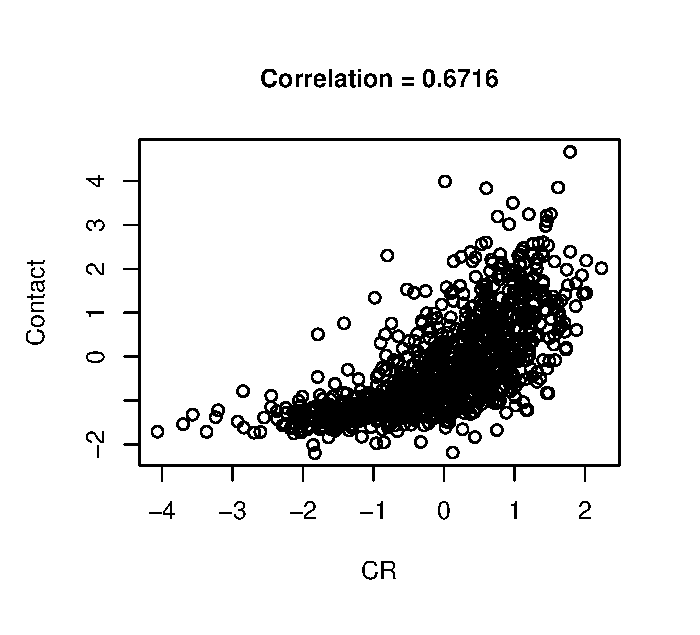
\includegraphics[width=.85\textwidth]{img/fsdm_results/contact_corr.eps}
\endminipage\hfill
\minipage{0.5\textwidth}
    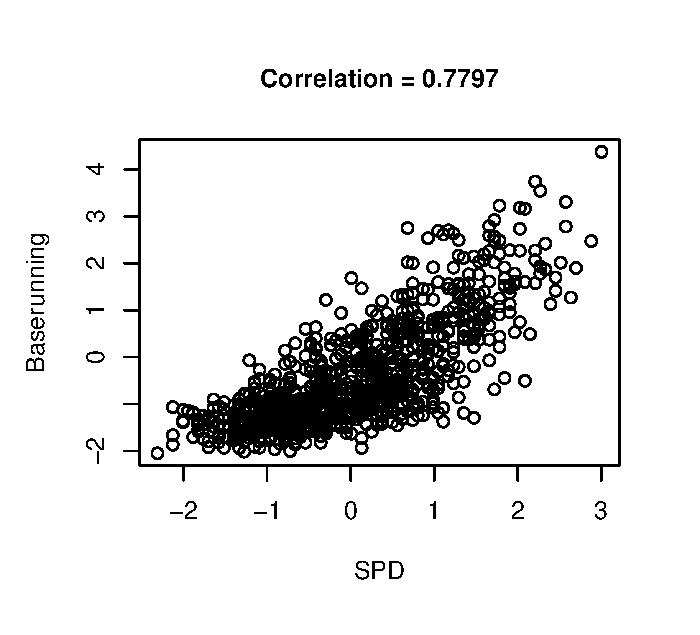
\includegraphics[width=.85\textwidth]{img/fsdm_results/baserun_corr.eps}
\endminipage
\hfill
\minipage{0.5\textwidth}
    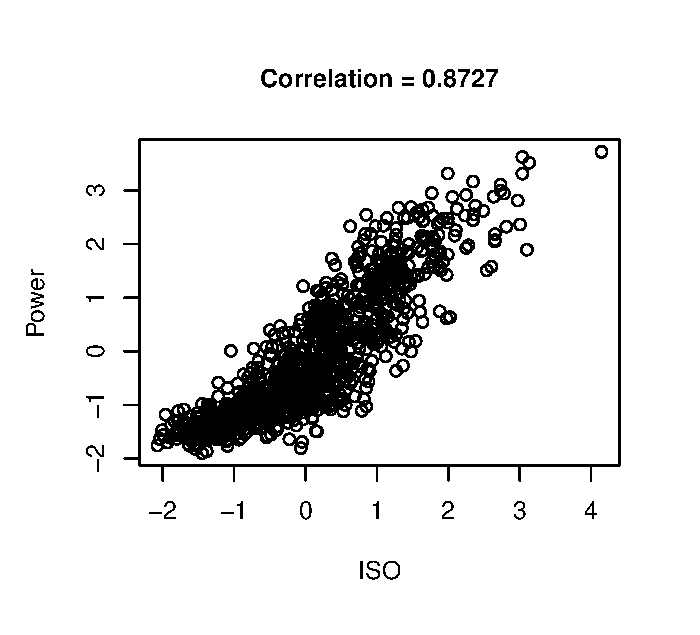
\includegraphics[width=.85\textwidth]{img/fsdm_results/power_corr.eps}
\endminipage\hfill
\minipage{0.5\textwidth}
    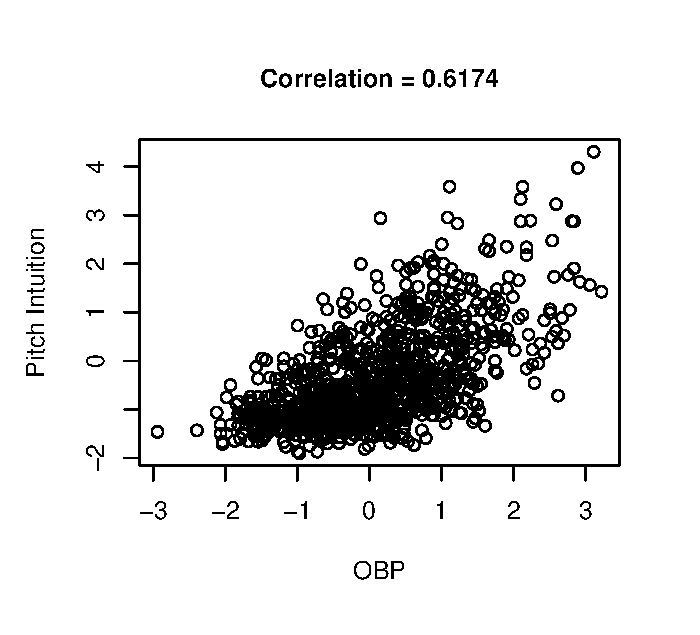
\includegraphics[width=.85\textwidth]{img/fsdm_results/pitch_intuit_corr.eps}
\endminipage\hfill
\caption{Each latent skill's estimates plotted against its evaluation statistic.}
\label{fig:baseball}
\end{figure*}

Each skill is plotted against its evaluation statistic in Figure \ref{fig:baseball} \cite{fsdm_paper}. Note that each of the four plots display high correlation, but do not match exactly. This is desirable in the sense that our new skill quantifications do in fact measure what they are intended to measure, but give new insights and ranking for each player. Though these results could be improved, it is clear that variations of the ML2P-VAE model can be applied in areas other than education.



\chapter{Knowledge Tracing Background}

Knowledge Tracing (KT) is a task introduced by Corbett and Anderson in 1995 \cite{corbett1995}. Their goal was to model the changing knowledge state of students as they progress through an online intelligent tutoring program. This tutoring system helps students practice writing computer programs by testing them on various rules, such as correct use of in-built functions, and providing feedback on their mistakes. The model tracks each student's knowledge as being in either a learned or unlearned state for each rule. After each interaction, there is a probability $P(T)$ that a student makes the transition from the unlearned state to the learned state.

The probability that a student has learned a particular rule at timestep $n$ is
\begin{equation}
P(L_n) = P(L_{n-1} | \text{evidence}) + (1 - P(L_{_n-1} | \text{evidence})) \cdot P(T).
\label{eq:kt}
\end{equation}
Then the probability of a student performing a task correctly is the sum of the probability that the rule is learned and the student doesn't make a mistake, and the probability that the rule is unlearned but the student guesses correctly.

There are only four parameters for each rule: the probability that the rule is already in the learned state at timestep 0, the probability of transitioning from the unlearned to learned state, the probability of guessing correctly, and the probability of slipping. These parameters are estimated using a hidden Markov Model, and the probability of a the student having learned a rule is updated via Bayes' Theorem.

In recent years, Bayesian Knowledge Tracing (BKT) has been overcome by deep learning methods. The popularity of neural networks has brought black-box models that yield high accuracy. Many of these methods, detailed in Section \ref{sec:kt_lit}, do not provide a concrete measure of student ability over time. Instead, the only way to track student knowledge is through the predicted probability of them answering questions correctly at a given timestep. 

In Chapter \ref{ch:kt_methods}, new methods using neural networks are presented which produce comparable predictive power to deep learning methods, while providing explainable models with links to Item Response Theory.


\section{Literature Review}\label{sec:kt_lit}
In the modern knowledge tracing application, data is provided as a sequence of student interactions $x_t = (q_t, c_t)$, $0 \leq t \leq L$. $L$ is a hyper-parameter denoting the maximum length of the sequence -- since the number of interactions for each student is different, response sequences shorter than $L$ are padded with null interactions, and response sequences of length longer than $L$ are wrapped into multiple sequences. For example, if $L=128$ and a particular student answers $160$ questions, then this student's interactions will be split into two separate sequences of length $128$ and $32$.

The tag $q_t$ indexes a particular question (item) in the available question bank, and $c_t \in\{0,1\}$ indicates whether the question was answered correctly or not. So for learning system with $n$ available questions, there are $2n$ possible interactions for $x_t$. The knowledge tracing task is to predict $c_{t+1}$ given all previous interactions. Mathematically, the quantity of interest is the probability 
\begin{equation}
  P(c_{t+1} = 1 | (q_0,c_0), (q_1,c_1),\ldots,(q_t, c_t), (q_{t+1}, ?)).
  \label{eq:kt_prob}
\end{equation}
Most neural networks optimize the predicted probability in Equation \ref{eq:kt_prob} by  minimizing the cross-entropy loss function, as described in Equation \ref{eq:cross_entropy}.

\subsection{Deep Knowledge Tracing}
In 2015, the first use of neural networks for knowledge tracing was introduced by Piech et al. \cite{piech2015}. Deep Knowledge Tracing (DKT) utilizes recurrent neural networks (RNN) and Long-Short Term Memory (LSTM) neural networks to predict a student's success on future questions, given a sequence of previous interactions. RNN are the most simple neural network to deal with sequential time-series data. \sideremark{Do I need to give background on RNN and LSTM?} LSTM are more sophisticated, and are capable of capturing longer-range dependencies due to their ``keep/forget'' functionality.

Similar to natural language processing, tokens (student interactions) need to be represented as a $d$-dimensional vector. DKT does this by one-hot encoding the interactions in the input layer of shape $(2n+1, L)$,  and linearly mapping to a hidden layer of shape $(d, L)$. Each interaction in the sequence is treated independently in this layer. The input layer shape is $2n+1$ for each of the possible $2n$ interactions, along with space for an additional padding token representing a null interaction (for response sequences of length $< L$.

  The architecture of DKT is as follows: The one-hot encoding input layer, the $d$-dimensional embedding, an LSTM layer of size $d$, and a feedforward output layer with $n$ nodes. The final layer uses a sigmoid activation function, and the output at each node represents the probability of answering that item correctly at the given timestep. To calculate loss, only the item tag for the next interaction and corresponding output node is used in the cross-entropy loss calculation.

\subsection{Dynamic Key-Value Memory Networks}
More sophisticated neural network approaches to knowledge tracing were introduced by Zhang et al. with Dynamic Key-Value Memory Networks (DKVMN) \cite{zhang2017}. They modify a memory-augmented neural network (MANN) in order to fit into the knowledge tracing framework. A MANN is a time-series neural network, but it does not rely on residual connections like an RNN or LSTM. Rather, a value matrix $M^v$ is stored in memory for each student, and the entries in $M^v$ are updated in each timestep. The predicted output is a probability dependent on the previous value of $M^v$ in timestep $t-1$, as well as the current neural network input in timestep $t$.

In DKVMN, there is some added interpretability by requiring the number of columns of $M^v$ to be equal to the number of knowledge concepts $K$. In this way, the columns of $M^v$ offer an $h$-dimensional representation of the student's skill. DKVMN splits the computations into two parts: \textit{read} from $M^v$ to make a prediction, and \textit{write} to $M^v$ to update its information. The predictive part inputs only an exercise tag $q_t$ without the true response $c_t$. The question tag is linearly embedded into a vector $k_t$. $k_t$ is a representation of question $q_t$, and is then multiplied by a learned matrix $M^k$ and softmaxed. 

This creates a vector $w_t$, where entry $j$ in $w_t$ represents the correlation weight between the question $q_t$ and memory slot $j$. This process of taking the dot product between an item embedding and a trainable matrix and softmaxing is similar to the concept of ``attention'', used in popular NLP techniques such as transformers \cite{vaswani2017}.

Next, \textit{read} from the value matrix by computing 
\begin{equation}
  r_t = \sum_{i=1}^K w_t(i) M^v(i).
  \label{eq:dkvmn_read}
\end{equation}
Note that $r_t$ is simply a weighted sum of the columns of $M^v$ and can be treated as a summary of the student's predicted master level of exercise $q_t$. Next, the item embedding $k_t$ is appened to the read content $r_t$ and fed forward through two linear layers. The first uses a $\tanh$ activation function, and the output $p_t$ produced a single node and a sigmoidal activation. In this way, the single value $p_t$ represents the probability that the student will answer item $q_t$ correctly at that timestep.

The second part of DKVMN is to \textit{write} new values into $M^v$ based on the true response of students. Different from the prediction phase, the full tuple $(q_t,c_t)$ is embedded into a vector $v_t$. The manner in which $M^v$ is updated is actually similar to that of an LSTM, allowing for ``remembering'' and ``forgetting''. Two trainable matrices are multiplied by $v_t$ to produce an ``erase`` vector $e_t$ and an ``add`` vector $a_t$. The erase vector has a sigmoidal activation function, so that values near zero do not get erased much at all, and values near 1 get erased quite a bit. The add vector uses a $\tanh$ activation function, so memory slots in $M^v$ can either be increased or decreased. Finally, the columns of the memory matrix are updated via
\begin{equation}
  M_{t}^v(i) = (M_{t-1}^v(i) [1 - w_t(i) e_t] ) + w_t(i) a_t
  \label{eq:update_dkvmn}
\end{equation}
Note that the correlation weights $w_t$ computed in the predictive step are again used to determine \textit{how much} of memory slot $i$ should be updated.

\sideremark{should I include image of DKVMN architecture?}

DKVMN's use of a matrix stored in memory allows for longer range dependencies than RNN or LSTM. There is also a bit of interpretability in this method, since a single column of the memory matrix $M_t^v$ gives an $h$-dimensional representation of a single skill for the student at time $t$. However, it cannot be determined \textit{which} skill the column represents. Additionally, if a student answers each available item, then stacking each weights vector $w_t$ into a matrix $W = \{w_t\}_{t=1}^L$ should result in a matrix similar to the item-skill association $Q$-matrix. But again, the columns of this ``learned $Q$-matrix'' $W$ are in no particular order, and can be difficult to interpret.

\subsubsection{Deep-IRT}
Don't need a lot of details here, but they modify DKVMN to gain connection with IRT

\subsection{Self-Attentive Knowledge Tracing}
Important just because this is used in KT-IRT

\subsection{Performance Factors Analysis}
*should explain more, because of deep-pfa (if that is included)




\chapter{Knowledge Tracing - Methods}

\section{Item-based Attention Networks}


\section{Deep Performance Factors Analysis}


\section{IRT Parameter Recovery + Knowledge Tracing}



\chapter{Comparison of Knowledge Tracing Methods}

\section{Data Description}\label{sec:kt_data}
We use four publicly available datasets, three of which are standard in the knowledge tracing literature. Two of the four datasets are simulated according to IRT models to demonstrate the capability of our IRT-inspired knowledge tracing methods to learn the IRT model parameters. We also include two real-world datasets common in knowledge tracing literature. A summary of each dataset is given in Table \ref{tab:kt_data}.

\subsubsection*{Synth-5}\footnote{https://github.com/chrispiech/DeepKnowledgeTracing/tree/master/data/synthetic}
This dataset was generated by Piech et al. \cite{piech2015} for experiments with DKT. There are 50 items covering 5 latent concepts. Each item requires exactly one concept, and responses are generated according to the Rasch model \cite{lord1968} with guessing: 
\begin{equation}
  P(u_{ij} = 1| \Theta_j; b_i) = c + \frac{1-c}{1 + e^{b_i - \theta_{jk}}}
  \label{eq:rasch_guess}
\end{equation}
The guessing parameter $c$ is fixed at $0.25$. Note that in Equation \ref{eq:rasch_guess}, only a single skill $k$ is referenced when answering item $i$. Responses to each of the 50 items are simulated for 4,000 students.

\subsubsection*{Sim200}\footnote{https://github.com/converseg/irt\_data\_repo/tree/master/sim200}
Sim200 differs from Synth-5 in a few important ways. First, there are more items (200) and more latent skills (20). Second, the $Q$-matrix is more dense -- items require multiple skills in order for students to answer correctly. Each entry in the $Q$-matrix was sampled from $\text{Bern}(0.2)$. Lastly, Sim200 generates responses according to the ML2P model in Equation \ref{eq:ml2p}, as opposed to the Rasch model. The item parameters were taken from a random uniform distribution; the difficulty parameters from $b_i \in [-3,3]$ and the nonzero discrimination parameters from $a_{ik} \in [0.1,0.9]$. This dataset is similar to the Sim-20 dataset described in Section \ref{sec:irt_data}, but the latent abilities $\Theta$ were generated according to a standard normal Gaussian distribution.

\subsubsection*{Statics2011}\footnote{https://pslcdatashop.web.cmu.edu/DatasetInfo?datasetId=507}
Statics is a real-world dataset with responses from 316 students enrolled in a college engineering course. After formatting the data, the dataset includes 987 unique items and 61 latent concepts. Students answered varying amounts of questions, with a total of 135,338 distinct interactions.

\subsubsection*{Assist2017}\footnote{https://sites.google.com/view/assistmentsdatamining}
The ASSISTments 2017 dataset contains real-world interactions from 1,709 students recorded on the ASSISTments online tutoring system. There is a large number of distinct items (4,117), and 102 latent concepts. Some items are tagged with the concept ``noskill'' -- we treat this tag as a latent concept, otherwise all interactions involving such items would need to be thrown out.

\begin{table}
  \centering
  \begin{tabular}{l c c c c}
    \hline
    Dataset & Items & Skills & Students & Interactions \\
    \hline
    Synth-5 & 50 & 5 & 4,000 & 20K \\
    Sim200 & 200 & 20 & 50,000 & 10M \\
    Statics2011 & 987 & 61 & 316 & 135K \\
    Assist2017 & 4,117 & 102 & 1,709 & 392K \\
  \end{tabular}
  \caption{Summary of datasets.}
  \label{tab:kt_data}
\end{table}


\section{Experiment Details}
In the two simulated datasets (Synth-5 and Sim200), all students answering the same set of questions and thus all have the same length of response sequences (50 and 200, respectively). On Statics2011 and Assist2017, the maximum sequence length is set at $L=128$, and student's whose response sequences are longer/shorter than 128 interactions have their response sequences wrapped/padded. The rest of the hyper-parameters are described in Table \ref{tab:kt_params}. The hyperparameters for DKT, SAKT, and DKVMN follow those reported in the corresponding literature.

\begin{table}
  \centering
  \begin{tabular}{l c c c c c}
    \hline
    Parameter & Synth-5 & Sim200 & Statics2011 & Assist2017 \\
    \hline
    max\_len & 50 & 200 & 128 & 128 \\
    input\_size & 101 & 201 & 1975 & 8235 \\
    output\_size & 50 & 200 & 987 & 4117 \\
    hid\_size & 64 & 64 & 50 & 100 \\
    skill\_layer & 5 & 20 & 61 & 102 
  \end{tabular}
  \caption{Hyper-parameters used in DKT-IRT and SAKT-IRT on each dataset.}
  \label{tab:kt_params}
\end{table}

\section{Results}

As seen in Table \ref{tab:kt_results}, the two IRT-inspired knowledge tracing methods methods (DKT-IRT and SAKT-IRT) are able to produce AUC values competitive with other deep learning methods. As expected, the sacrifice in accuracy is smaller in simulated datasets. In Synth-5 and Sim200, the responses were generated with known IRT models which match the architecture of IRT-inspired methods. 

\begin{table}
  \centering
  \begin{tabular}{l c c c c}
    \hline
    Method & Synth-5 & Sim200 & Statics2011 & Assist2017 \\
    \hline 
    DKT & 0.803 & 0.838 & 0.793 & 0.731 \\
    SAKT & 0.801 & 0.834 & 0.791  & 0.754 \\
    DKVMN & 0.827 & 0.829 & 0.805 & 0.796 \\
    \textbf{DKT-IRT} & 0.799 & 0.824 & 0.777 & 0.724 \\
    \textbf{SAKT-IRT} & 0.798 & 0.833 & 0.775 & 0.728
  \end{tabular}
  \caption{TestAUC values for various models on each dataset.}
  \label{tab:kt_results}
\end{table}

Note that when working on Synth-5, we know that there were no discrimination parameters used to generate the data. As such, we fix all nonzero weights in the output layer to be equal to one by replacing Equation \ref{eq:weight_constraint} with $W_p = Q$. We do not incorporate any estimation or knowledge of the guessing parameter $c$ into the knowledge tracing model. This may account for a larger discrepancy in AUC between our methods and DKVMN in Synth-5 than seen in the Sim200 data.

When looking at the two real-world datasets, the trade-off in AUC is more significant, as it is not known if the student responses follow the ML2P model. There could also be inaccuracies in the given item-skill association $Q$-matrix, which our models are dependent on. Additional difficulties arise in the Assist2017 data, discussed in Section \ref{sec:kt_data}, concerning exercise-skill tags may explain the considerable performance gap between IRT-inspired methods and DKVMN on this dataset.

\begin{figure}[h]
  \centering
  \includegraphics[width=.5\textwidth]{img/kt_irt/synth5_diff_est_lstm.png}
  \caption{Correlation between DKT-IRT estimates and true values of Synth-5 item difficulty. SAKT-IRT produced similar results.}
  \label{fig:synth5_diff}
\end{figure}

A comparison between the output layer bias parameters and true item difficulty parameters is shown in Figure \ref{fig:synth5_diff}. This displays high correlation, and the trainable bias parameters in the output layer can be interpreted as approximations of the item difficulty parameters. Due to the available public dataset, there is no access to the true values of student abilities $\Theta$.

\begin{figure}[h]
  \centering
  \minipage{.5\textwidth}
  \includegraphics[width=.85\textwidth]{img/kt_irt/disc_est_attn2.png}
  \endminipage
  \minipage{.5\textwidth}
  \includegraphics[width=.85\textwidth]{img/kt_irt/diff_attn_sim200.png}
  \endminipage
  \caption{Correlation between true and estimated Sim200 (left) item discrimination parameters, and (right) item difficulty parameters.}
  \label{fig:disc_diff_sim200}
\end{figure}

The parameter estimates can be directly compared to the true parameters in the Sim200 dataset. In Figure \ref{fig:disc_diff_sim200}, we can see the true values of item discrimination parameters $a_{ik}$ and item difficulty parameter. The correlation here is very high, and the estimates for item parameters are quite accurate. The student ability parameters $\theta_{jk}$ plotted against estimates given by SAKT-IRT at the final timestep in Figure \ref{fig:theta_sim200}. While there is a lot more noise in the student ability estimates, there is still significant correlation with the true values. 

It is important to note that the estimates to $\Theta$ do not require any additional computations or transformations and are directly obtained from the nerual network. This is an advantage over other deep knowledge tracing methods, which only output the probability of answering items correctly and require other methods of quantifying knowledge concepts. Recall that while estimates to student ability are the neuron activation values at the skill layer from feeding forward a response sequence, the discrimination parameter estimates are the trained weights connecting the skill layer to the output layer.

\begin{figure}[h]
  \centering
  \includegraphics[width=.5\textwidth]{img/kt_irt/theta_est_attn2.png}
  \caption{Correlation between true and estimated student ability parameters at $t=L=200$ for the Sim200 dataset.}
  \label{fig:theta_sim200}
\end{figure}

\begin{figure}[h]
  \centering
  \includegraphics[width=.7\textwidth]{img/kt_irt/knowledge_trace_lstm_edited.png}\\
  \vspace{.5cm}
  \includegraphics[width=.7\textwidth]{img/kt_irt/knowledge_trace_attn_edited.png}
  \caption{Tracing a student's knowledge mastery with DKT-IRT (top) and SAKT-IRT (bottom) as they progress through the items of the Synthetic-5 dataset.}
  \label{fig:synth5_trace}
\end{figure}

The explcit representation of knowledge $\Theta$ makes tracing student progress over time very convenient. For student $j$'s response sequence of length $L$, IRT-inspired knowledge tracing methods return a $K \times (L+1)$ matrix, where the entry $(k,t)$ gives the latent trait estimate to the $k$-th skill at time $t$, $\theta_{jkt}$. This is visualized in Figure \ref{fig:synth5_trace} on the Synth-5 dataset. Notice how a correct response in a skill (filled-in circle) corresponds with a more green and less red skill value. Likewise, an incorrect response in a skill (hollow circle) corresponds with a more red skill or less green skill value. When comparing the knowledge tracing from DKT-IRT and SAKT-IRT, the DKT-IRT tracing is much more smooth as a student moves through the exam. This is likely because of the recurrent structure of an LSTM: the skill values at time $t$ are only directly related to the values at time $t-1$. The SAKT-IRT tracing graphic is much choppier, because the attention mechanism does not have recurrent structure and instead maintains connections to all previous interactions.


\section{Discussion}
The connection between IRT and knowledge tracing presented in this work introduces a trade-off between accuracy and interpretability. Further work to increase AUC to the level of DKVMN while maintaining explainability is worth exploring. Though IRT-inspired knowledge tracing does require an expert to annotate the item-skill association $Q$-matrix while other methods do not, explicitly incorporating this information greatly increases the ability to interpret a deep learning model. Further, most intelligent tutoring systems provide an item-skill tag, so availability of the $Q$-matrix is not an unreasonable assumption.

Our proposed method's ability to function as both a knowledge tracing model while also estimating item parameters gives it a unique interpretation rooted in Item Response Theory. This link with IRT is helpful in practice, because it provides an explicit and easy to obtain quantity for a student's latent abilities. This approximation of a student ability can be interpreted in the frame of IRT, as opposed to only a prediction of correctness for each item. This is a clear advantage that IRT-inspired knowledge tracing has over conventional non-interpretable deep learning methods.


%\include{chapter2}
%\include{chapter3}
%\include{chapter4}
%\include{chapter5}
%\include{chapter6}
%% !Tex root = thesis.tex

% Appendices
\appendix \label{apdx}

%\chapter{Glossary of Notation}


\chapter{Artificial Neural Networks} \label{apdx:ann}
Artificial Neural Networks (ANN) are commonly understood to be complicated black box machine learning methods which produce high levels of accuracy, while sacrificing interpretability \cite{pattern_rec_book}. This assessment is true in part -- the end-to-end decision process of a trained neural network is very convoluted. But after zooming in to the inner workings of an ANN, each individual part is quite simple.

\section{Architecture}
Neural networks have a graph-like structure with vertices (nodes) and weighted edges. A basic feed-forward neural network (FFN) consists of an input layer, a number of hidden layers, and an output layer. A ``layer'' $l$ consists of $n_l$ nodes, and each node $i$ is densely connected to every node in the previous layer $l-1$ by a weighted edge. In this manner, the subgraph containing all nodes of layer $l-1$ and all nodes of layer $l$ can be seen as a complete bipartite graph $K_{n_{l-1}, n_l}$. A simple FFN is shown in Figure \ref{fig:ffn_example} which takes inputs with 10 features and classifies into three categories \cite{nn_svg}. For example, inputs could represent the weight, height, hair length, etc. of a pet, with the task of classifying the pet as a cat, dog, or bird \cite{neural_net}.

\begin{figure}[h]
  \centering
  \includegraphics[width=.85\textwidth]{img/ffn_visual.png}
  \caption{A basic FFN with input size $n_0 = 10$ and output size $n_3 = 3$, with two hidden layers of size $n_1 = 5$ and $n_2 = 6$.}
  \label{fig:ffn_example}
\end{figure}

While the architecture of a neural network can be described using the lens of graph theory, the inner workings are better explained using basic linear algebra. Each layer acts as a function from $\R^{n_{l-1}}$ to $\R^{n_{l}}$. Specifically, this function is a linear transformation followed by a nonlinear rescaling. For a given input vector $\vect x^* \in \R^{n_0}$ and its corresponding true label $\vect y^*$, the value in the first hidden layer is calculated as
\begin{equation}
  \vect a_1^* = f_1(W_1 \vect x^* + \vect b_1)
  \label{eq:hid_layer}
\end{equation}
where $W_1 \in \R^{n_1 \times n_0}$ and $\vect b_1 \in\R^{n_1}$ are the trainable \textit{weights} matrix and \textit{bias} vector. The notion of ``trainable'' parameters is explored further in Appendix \ref{apdx:backprop}. The value $\vect a_1^*$ is called the \textit{activation} value of the input $\vect x^*$ at hidden layer $l=1$. The non-decreasing function $f_1$ is called an \textit{activation function} which applies a (possibly) non-linear rescaling to the vector $\vect z_1^* = W_1 \vect x^* + \vect b_1 \in \R^{n_1}$ element-wise. Examples of different activation functions are given in Appendix \ref{apdx:activation_fcns}. Matrix notation can also be abandoned by writing the activation of the $i$-th node in layer $l=1$ as 
\begin{equation}
  a_{1,i}^* = f_1\left(b_{1,i} + \sum_{j=1}^{n_0} w_{ij}^1 \cdot x_j^* \right)
  \label{eq:element_activation}
\end{equation}
where $w_{ij}^1$ is the element in the $i$-th row and $j$-th column of $W_1$, the weight connecting the $j$-th node of layer $0$ to the $i$-th node of layer $1$.

The activation value of the input $\vect x^*$ at hidden layer $l=2$ and the output layer $l=3$ can similarly be computed as
\begin{equation}
  \begin{split}
    \vect a_2^* &= f_2(W_2 \vect a_1^* + \vect b_2) \\
    \hat{\vect y}^* &= \vect a_3^* = f_3(W_3 \vect a_2^* + \vect b_3)
  \end{split}
  \label{eq:ffn_comp}
\end{equation}
where the weights matrices $W_2 \in \R^{n_2 \times n_1}$ and $W_3 \in \R^{n_3 \times n_2}$ and bias vectors $\vect b_2 \in \R^{n_2}$ and $\vect b_3 \in \R^{n_3}$ are trainable. Before training, all trainable parameters are typically initialized randomly. The output value $\hat{\vect y}^*$ serves as the prediction for input $\vect x^*$. 

For classification, the true label $\vect y$ is often a one-hot encoding, so the prediction $\hat{\vect y}^*$ should be a probability distribution each entry describes the certainty of the model in classifying the input $\vect x^*$ as each possible class. Returning to the earlier example, an input with features pertaining to a cat has the true label $(1,0,0)$. An output prediction may give $(0.65, 0.32, 0.03)$, meaning that the neural network is $65\%$ confident that the input features are that of a cat, $32\%$ confident that the input is a dog, and $3\%$ confident that the input is a bird.

\section{Activation Functions} \label{apdx:activation_fcns}
The main purpose of activation functions is to rescale each layer so that every activation value falls in the same range. Performing many matrix multiplications in a row can easily cause values to become very large, leading to over-fitting and other complications \cite{sibi2013}. It can be helpful to use an activation function to map values to the range of $(0,1)$ because of the effect of the numbers $0$ and $1$ in multiplication, map to $(-1,1)$ to utilize positive and negative values, or map to $[0,\infty)$ to avoid negative values. 

Though custom activation functions can be defined and easily implemented, below are a few examples of popular activation functions used in neural networks \cite{tensorflow} \cite{keras_r}. Each of these are independently applied to a vector element-wise, except for the softmax function which maps an $n$-dimensional vector to a discrete probability distribution with $n$ possible values. Denote $z = \sum_k a_k w_k + b$ as the input to a node's activation function.

\begin{equation}
  \text{Sigmoid: } \sigma(z) = \frac{1}{1 + e^{-z}} \quad \quad \R \to (0,1) 
  \label{eq:sigmoid_eqn}
\end{equation}
The sigmoid activation function has the form of the logistic curve and maps values to be between $0$ and $1$.

\begin{equation}
  \text{Hyperbolic tangent: } \tanh(z) = \frac{e^z - e^{-z}}{e^z + e^{-z}} \quad \quad \R \to (-1,1)
  \label{eq:tanh_eqn}
\end{equation}
Hyperbolic tangent has a similar curvature to that of the sigmoid, but maps values to between $-1$ and $1$. 

\begin{equation}
  \text{Rectified Linear Unit (ReLU): } \text{relu}(z) = \max\{0, z\} \quad \quad \R \to (0,\infty)
  \label{eq:relu_eqn}
\end{equation}
The ReLU function is often used to combat the ``learning slowdown'' problem that the sigmoid and $\tanh$ can face -- if an input $z_0$ is very large or very small, then the derivative $\displaystyle\frac{d\sigma}{dz} \Big|_{z=z_0}$ is very small, causing gradient descent iterations to improve slowly. The derivative of the ReLU function is either exactly 0 or exactly 1, which helps speed up the training process.

\begin{equation}
  \text{Softmax: } \text{softmax}(\vect z)_i = \frac{e^{z_i}}{\sum_{j=1}^n e^{z_j}} \quad \quad \R^n \to \{P(x=i)\}_{i=1}^n
  \label{eq:softmax_eqn}
\end{equation}
When using the softmax activation function, the activation a single node is a function of the activation of all other nodes within the same layer. This is seen in the summation over $n$ nodes in Equation \ref{eq:softmax_eqn}. It is also straightforward to see that for any input, the sum of all $n$ nodes in the layer always adds up to exactly 1 -- so a softmax layer with $n$ nodes can be understood as a discrete probability distribution with $n$ classes. This can be particularly useful in the output layer of a multi-class classification neural network model.


\section{Optimization and Backpropagation}\label{apdx:backprop}
Figure \ref{fig:ffn_example} and Equations \ref{eq:hid_layer} and \ref{eq:ffn_comp} show that given an input $\vect x^*$, a feed-forward neural network can output a prediction $\hat{\vect y}^*$. We now turn to the way in which $\hat{\vect y}^*$ serves as a \textit{quality} prediction of the true value $\vect y^*$. The terminology of ``training'' a neural network refers to finding optimal settings of the weights matrices $W_l$ and bias vectors $\vect b_l$ in each layer $l$ which minimize the error between predictions $\hat{\vect y}^*$ and true inputs $\vect y^*$. Such measures of error are called \textit{loss functions}.

Though there are many candidates for loss functions such as cross-entropy (see Equation \ref{eq:cross_entropy}) or hinge loss \cite{gentile1998}, consider the simple mean squared-error loss function
\begin{equation}
  \mathcal{L}(\vect y, \hat{\vect y}) = ||\vect y - \hat{\vect y}||_2^2 = \frac{1}{K} \sum_{k=1}^K (y_k - \hat{y}_k)^2
  \label{eq:mse_loss}
\end{equation}
where $K$ is the dimension of the target (i.e. the number of output nodes).

Recall that if an input (or set of inputs) $\vect x^*$ is fixed, then the prediction $\hat{\vect y}^*$ outputted by the neural network is a function of the weights and biases $W_l$ and $\vect b_l$. As such, we can compute partial derivatives of $\mathcal{L}$ with respect to each trainable parameter and use a gradient descent algorithm to minimize Equation \ref{eq:mse_loss}.

Though deep neural networks can have thousands, millions, or billions of parameters \cite{gpt3}, calculating gradients remains feasible because of the backpropagation algorithm \cite{rojas1996}. While obtaining predictions from a neural networks works in a left-to-right fashion ($\vect a_3$ depends on $\vect a_2$, which depends on $\vect a_1$, which depends on $\vect x$), gradient calculations are computed right-to-left. This is due to the role of the chain rule.

First consider calculating the partial derivative of a particular weight in the final layer, $w_{ij}^3$. Denote the input to an activation function at layer $l$ as $\vect z_l = W_l \vect a_{l-1} + b_l$ so that $\vect a_l = f_l(\vect z_l)$. Using Equation \ref{eq:ffn_comp}, we can write
\begin{equation}
\frac{\partial \mathcal{L}(\vect y, \vect a_3)}{\partial w_{ij}^3} = \frac{\partial \mathcal{L}(\vect y, \vect a_3)}{\partial a_{3,i}} \cdot \frac{\partial a_{3,i}}{\partial z_{3,i}} \cdot \frac{\partial z_{3,i}}{\partial w_{ij}^3} = \frac{\partial \mathcal{L}(\vect y, \vect a_3)}{\partial a_{3,i}} \cdot f_3'(z_{3,i}) \cdot a_{2,j} 
  \label{eq:chain_rule}
\end{equation}
Now consider the change in loss with respect to a trainable parameter in the second-to-last layer. Choose a weight $w_{jk}^2$ whose right endpoint is the same node as the left endpoint of $w_{ij}^3$ used in Equation \ref{eq:chain_rule}. We have
\begin{equation}
  \begin{split}
    \frac{\partial \mathcal{L}(\vect y, \vect a_3)}{\partial w_{kj}^2} &= \sum_{i=1}^K \left(\frac{\partial \mathcal{L}(\vect y, \vect a_3)}{\partial a_{3,i}} \cdot \frac{\partial a_{3,i}}{\partial z_{3,i}} \cdot \frac{\partial z_{3,i}}{\partial a_{2,j}}\right) \cdot \frac{\partial a_{2,j}}{\partial z_{2,j}} \cdot \frac{\partial z_{2,j}}{\partial w_{jk}^2} \\
    &= \sum_{i=1}^K \left(\frac{\partial \mathcal{L}(\vect y, \vect a_3)}{\partial a_{3,i}} \cdot f_3'(z_{3,i}) \cdot w_{ij}^3 \right) \cdot f_2'(z_{2,j}) \cdot a_{1,k}
\end{split}
  \label{eq:chain_rule2}
\end{equation}

Notice how in Equation \ref{eq:chain_rule2}, information first calculated in Equation \ref{eq:chain_rule} is re-used. Particularly, the partial derivative of a parameter found in layer $l$ is a sum of partial derivatives of values found in layer $l+1$. In this sense, the backpropagation algorithm works right-to-left; first calculating values in layer $L$ that will later be used in all layers $l<L$.

After the gradient of $\mathcal{L}$ is found using backpropagation, a gradient descent update is performed for an input $\vect x$:
\begin{equation}
  \vect \Lambda_{t+1} \gets \vect \Lambda_{t} - \eta \nabla_{\vect \Lambda} \mathcal{L}(\vect y, \hat{\vect y})
  \label{eq:grad_update}
\end{equation}
where $\vect \Lambda$ is a vector containing all trainable parameters $W_l$ and $\vect b_l$ and $\eta$ is the learning rate hyperparameter \cite{ruder2017}. This process is repeated iteratively using randomly selected inputs $\vect x$ from the training set until convergence, as in the stochastic gradient descent (SGD) method. 


\chapter{\textbf{ML2Pvae} Package Details} \label{apdx:software}
In this section, we provide a tutorial of the \textbf{ML2Pvae} software package for R. Functions and data which are exported by the package are listed in {\color{blue}\verb!blue!}. This tutorial uses a simulated dataset which is accessible through the package, including:
\begin{itemize}
  \item A $Q$-matrix ({\color{blue}\verb!q_matrix!}) relating $n = 30$ items to $K = 3$ latent skills
  \item A covariance matrix ({\color{blue}\verb!correlation_matrix!}) detailing the correlations between the latent skills
  \item A set of $N = 5,000$ binary responses ({\color{blue}\verb!responses!}) to $n = 30$ items, generated by the ML2P model with true parameters:
    \begin{itemize}
      \item $\vect \Theta_j \in \R^3$, $1\leq j \leq 5,000$ ({\color{blue}\verb!theta_true!})
      \item $\vect a_i \in \R^3$, $1\leq i \leq 30$ ({\color{blue}\verb!disc_true!})
      \item $b_i\in \R$, $1\leq i \leq 30$ ({\color{blue}\verb!diff_true!}) 
    \end{itemize}
\end{itemize}

The \textbf{ML2Pvae} package has five easy-to-use functions to assist in building, training, and evaluating ML2P-VAE models. The functions {\color{blue}\verb!build_vae_independent()!} and {\color{blue}\verb!build_vae_correlated()!} construct a modified VAE architecture as specified by the user. The former assumes that the latent traits are independent ($\vect \Theta \sim \mathcal{N}(0,I)$), and the latter assumes knowledge of correlated latent traits ($\vect \Theta \sim \mathcal{N}(\vect \mu, \Sigma)$), as described in Section \ref{sec:cov}.

To train a VAE on a dataset, the function {\color{blue}\verb!train_model()!} can be used. After the model has been fitted, the function {\color{blue}\verb!get_item_parameter_estimates()!} grabs the relevant trainable weights from the decoder which serve as estimates of $\vect a_i$ and $b_i$. The function {\color{blue}\verb!get_ability_parameter_estimates()!} feeds student responses through the encoder to obtain estimates to $\vect \Theta_j$.

The functionality of \textbf{ML2Pvae} is displayed below. Note that while the neural network models are created with Tensorflow and Keras \cite{keras_r} inside of \textbf{ML2Pvae}, those packages are not employed by the user. This is by design in order to make the ML2P-VAE method accessible to IRT researchers in psychometrics who may not have knowledge of neural networks. Further explanation and documentation for \textbf{ML2Pvae} can be found at {\color{violet}\href{https://cran.r-project.org/web/packages/ML2Pvae}{https://cran.r-project.org/web/packages/ML2Pvae}}. Source code of the software is found at {\color{violet}\href{https://github.com/converseg/ML2Pvae}{https://github.com/converseg/ML2Pvae}}.

\section{Software Tutorial}
\vspace{.5cm}

%\lstset{language=R, keywords={}, otherkeywords={build\_vae\_independent, build\_vae\_correlated, train\_model, get\_item\_parameter\_estimates, get\_ability\_parameter\_estimates, responses, q\_matrix, correlation\_matrix, disc\_true, diff\_true, theta\_true}}
\lstinputlisting{ml2pvae_tutorial.R}
\begin{figure}[h]
  \centering
  \includegraphics[width=.95\textwidth]{img/ml2pvae_tutorial_plots.png}
  \caption{Correlation plots of IRT parameter estimates produced by the above code tutorial.}
  \label{fig:tutorial_plots}
\end{figure}








%
% this command includes the entire bib file in the
% references section, whether the entry has been
% cited in the paper or not
%
%\nocite{*}

\biblio{thesis}



\bibliographystyle{plain}
%\bibliography{thesis} % I guess this makes citations work?

%\singlespacing

\end{document}
